The lines are analysed as 550m sampling distance. (1:5 sub-sampling) and 5.5km (1:50 sub-sampling) sampling distance. The re-sampling is combined with a low-pass filter through rolling average and suggest the accuracy of the method for global low-resolution data. 

For the on-line detection a wait time of 80 samples was used \cite{Adams2007}. The Off-line detection used constant prior and full covariance model. Truncation at -100. \cite{Xuan2011,Xuan2007,Fearnhead2006}. \\

The run time for all results in this report, was 672s  in a parallel build on 6 cores. 2.6 GHz Intel Core i7, 16Gb. 

Maps are generated in QGIS, but colour maps is trivial and names refers to Geo-science Australia terrain map, as also used as references in the figures. 

\begingroup
\let\clearpage\relax
\listoffigures
\endgroup

\begin{figure}[h]
	\centering
	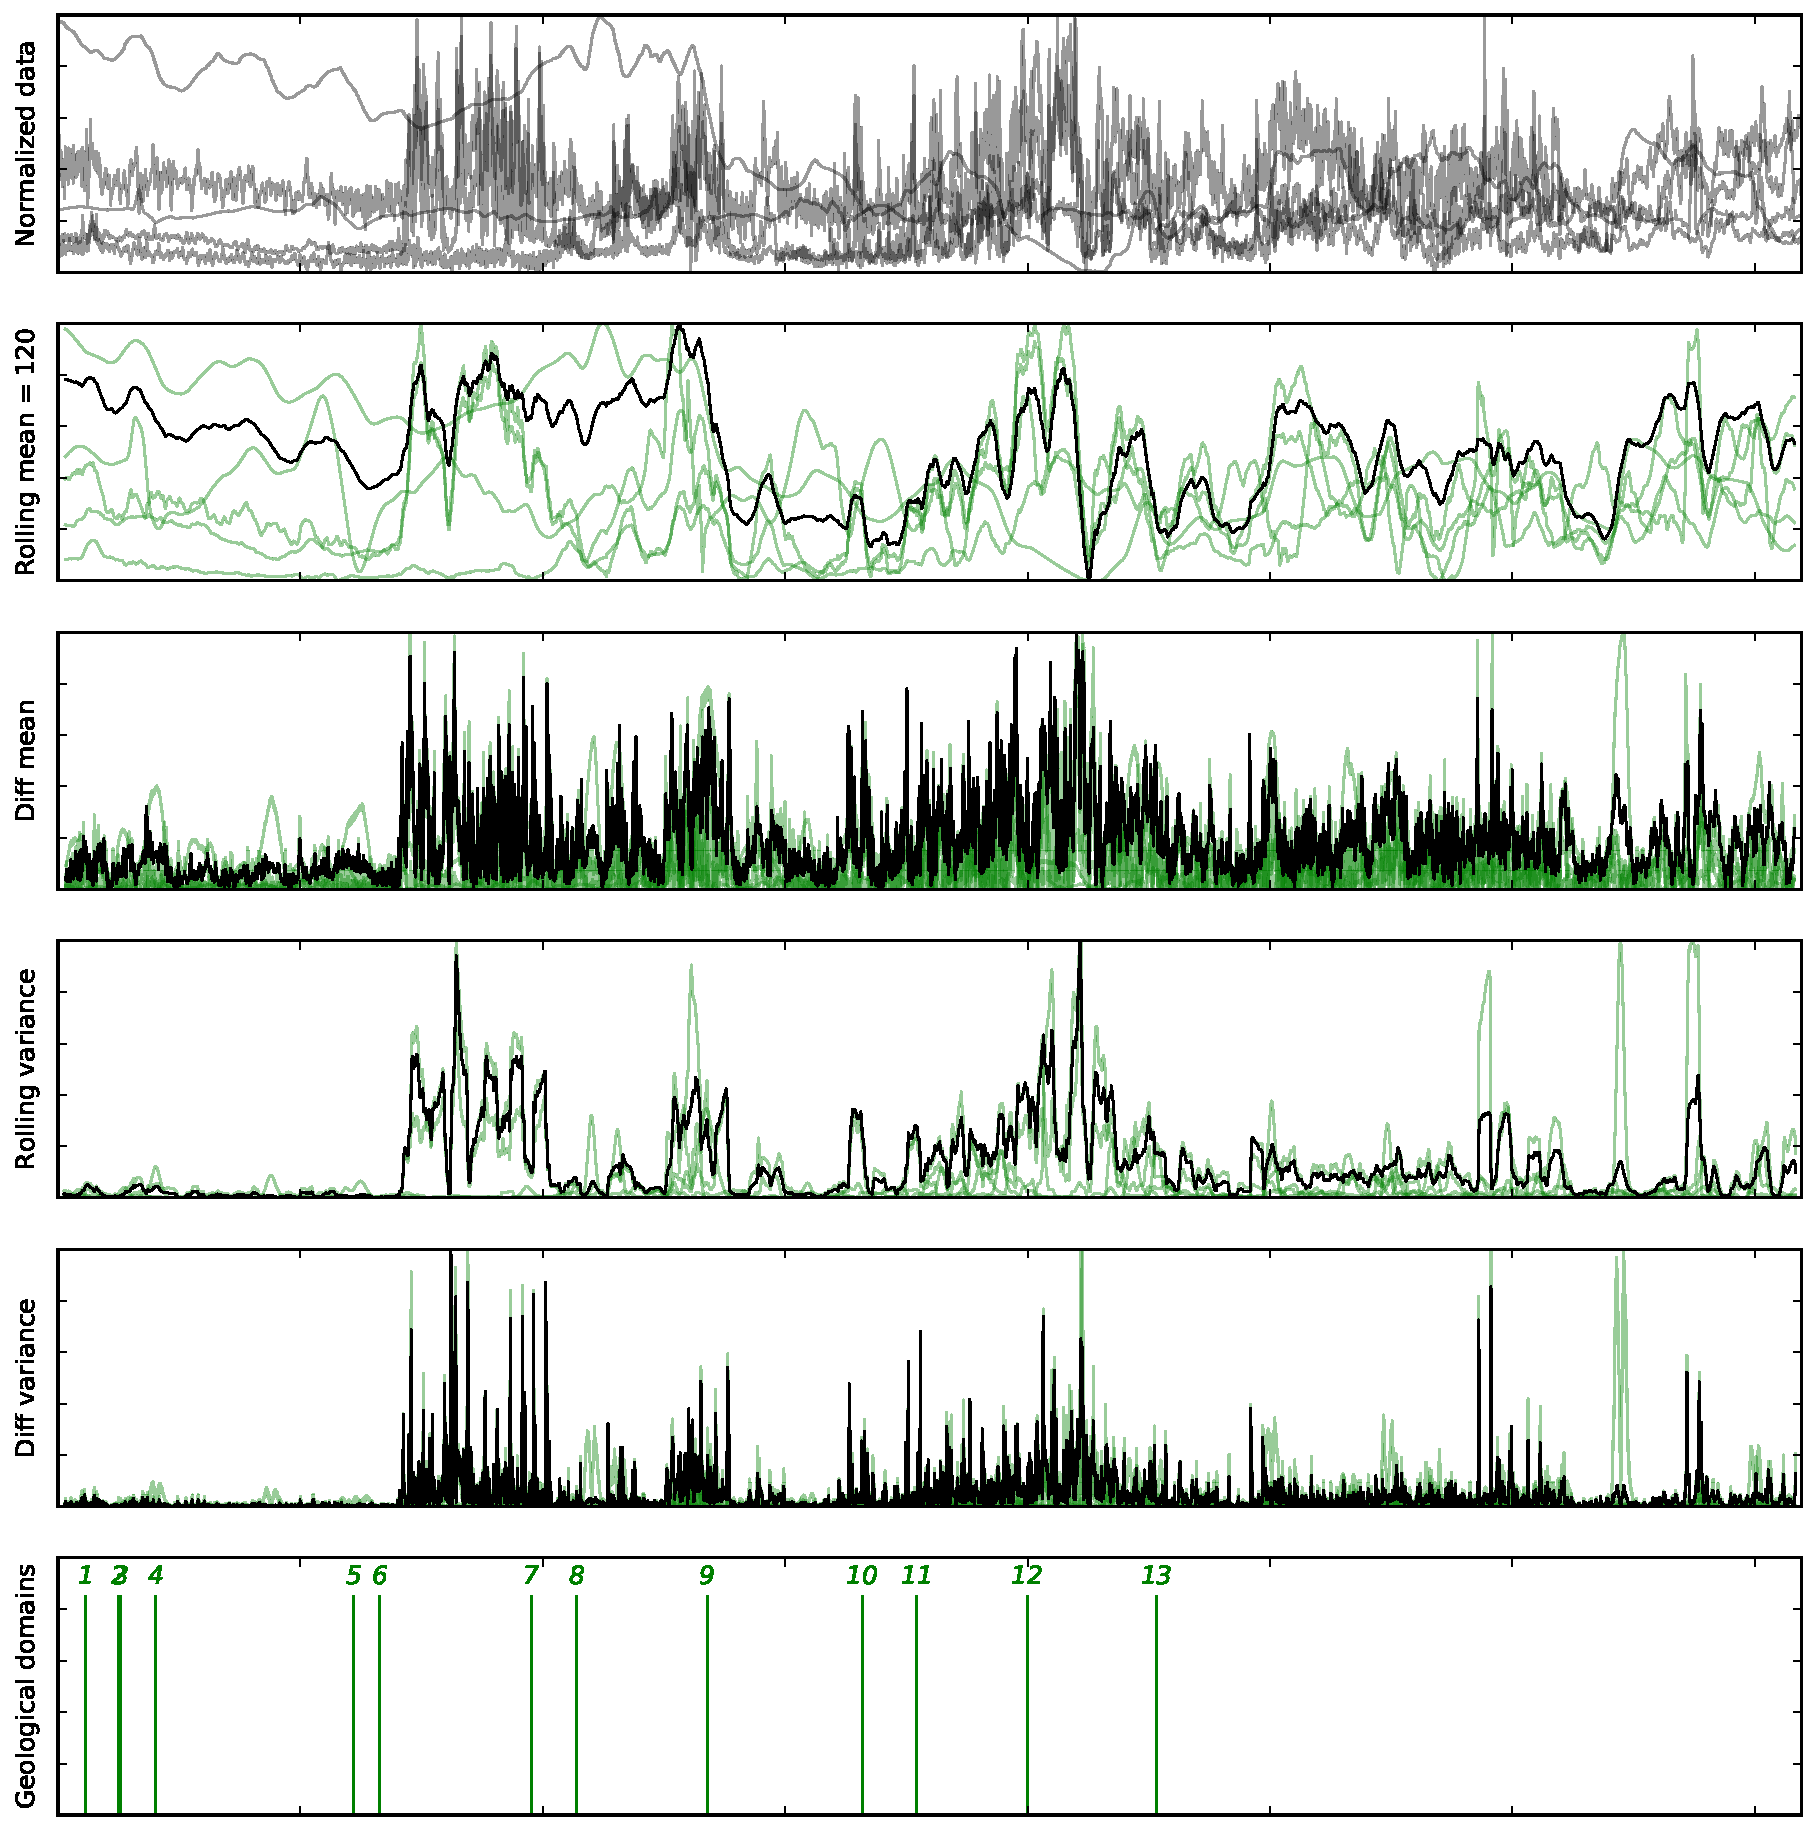
\includegraphics[width=1\linewidth]{../fig/naive_ga_vpt_line_2}
	\caption[Naïve 2]{Statistic analysis of Line 2. From left: Oscar Range region, basement province, 1: Nookanbah (250k) region, basement province, 2: Basement to Barbwire Terrace of 017 Canning Basin, 3: Lagrange (250k map) region, basement province, 4: Koop 100k map region (geophysicallly overprinted zone); basement province, 5: Roeves (gravity feature, Reeves Knoll) region; basement province, 6: 067 Paterson Province, 7: Rudall Inlier within  067 Paterson Province, 8: LD Lake Dissapointment  region (Gunanya 1:250k map); 067 Paterson Province (?), 9: Capricorn East (geophysical) region of Capricorn Orogen (e.g., Trainor 100k map); basement province (poorly defined), 10: Basement to 011 Bangemall Basin; Capricorn Orogen, 11: Overlies NE Yilgarn, 12: 093 Yilgarn Craton (Super)-province (Block)
}
	\label{fig:naive2}
\end{figure}


\begin{figure}[h]
	\centering
	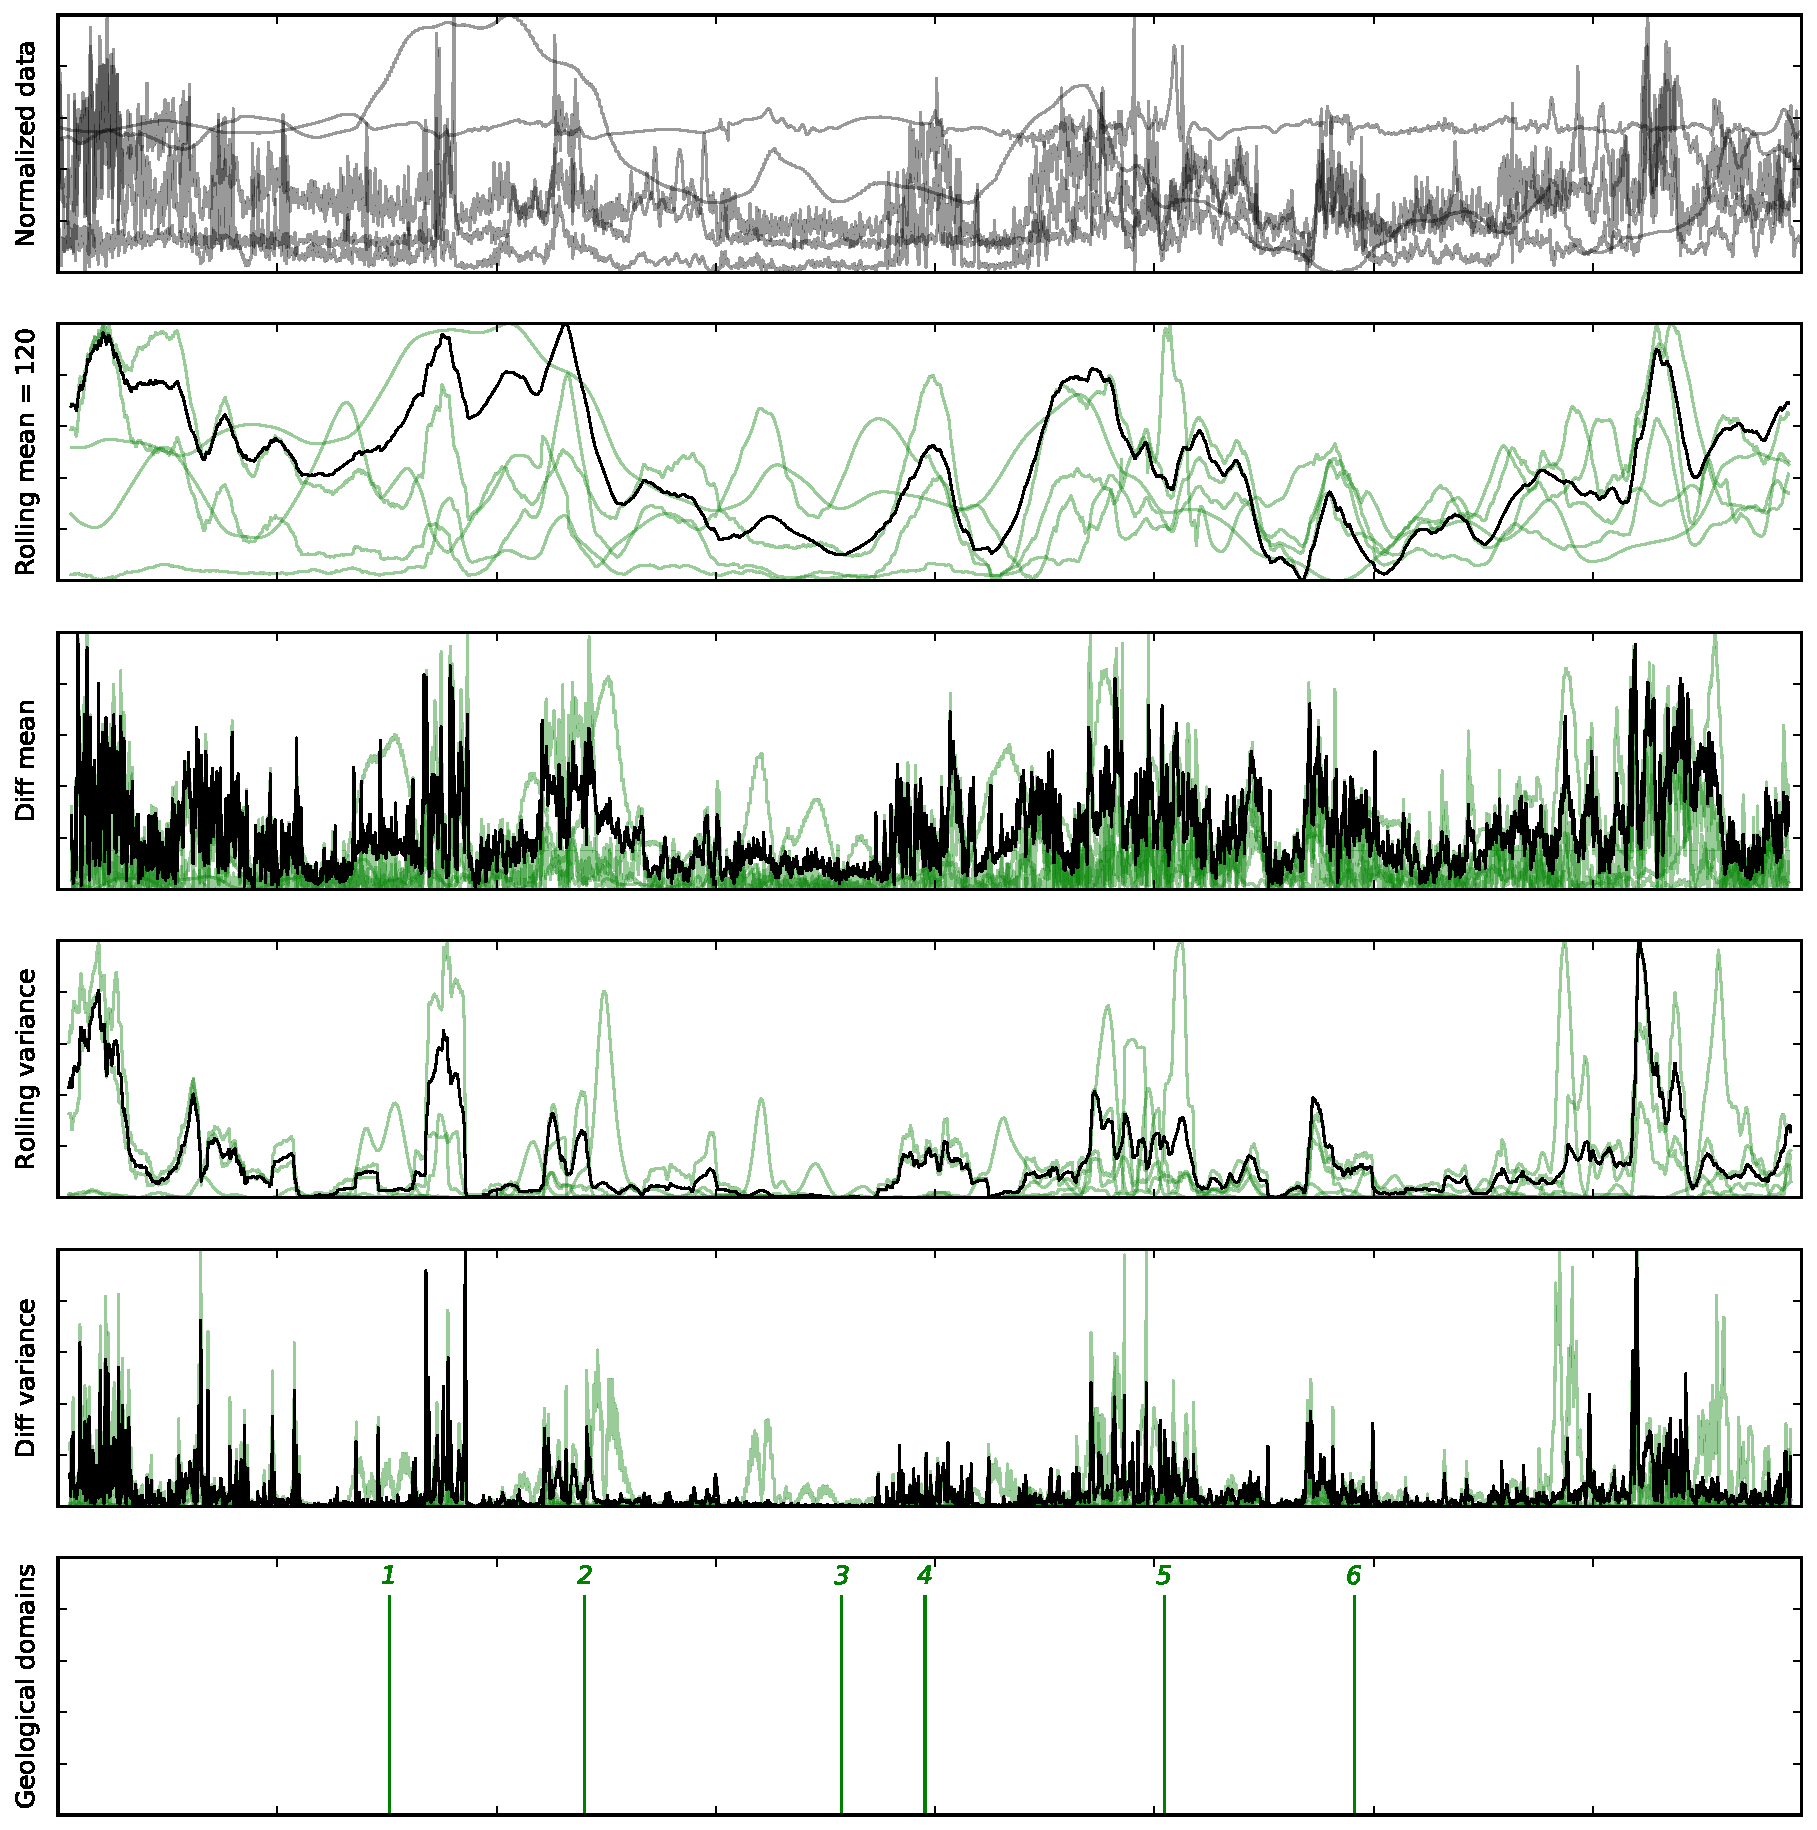
\includegraphics[width=1\linewidth]{../fig/naive_ga_vpt_line_15}
	\caption[Naïve 15]{Statistic analysis of Line 15. From left: Roeves (gravity feature, Reeves Knoll) region; basement province, 1: Rudall Inlier within  067 Paterson Province, 2: LD Lake Dissapointment  region (Gunanya 1:250k map); 067 Paterson Province (?), 3: Capricorn East (geophysical) region of Capricorn Orogen (e.g., Trainor 100k map); basement province (poorly defined), 4: Basement to 011 Bangemall Basin; Capricorn Orogen, 5: Overlies NE Yilgarn, 6: 093 Yilgarn Craton (Super)-province (Block)
}
	\label{fig:naive15}
\end{figure}

\begin{figure}[h]
	\centering
	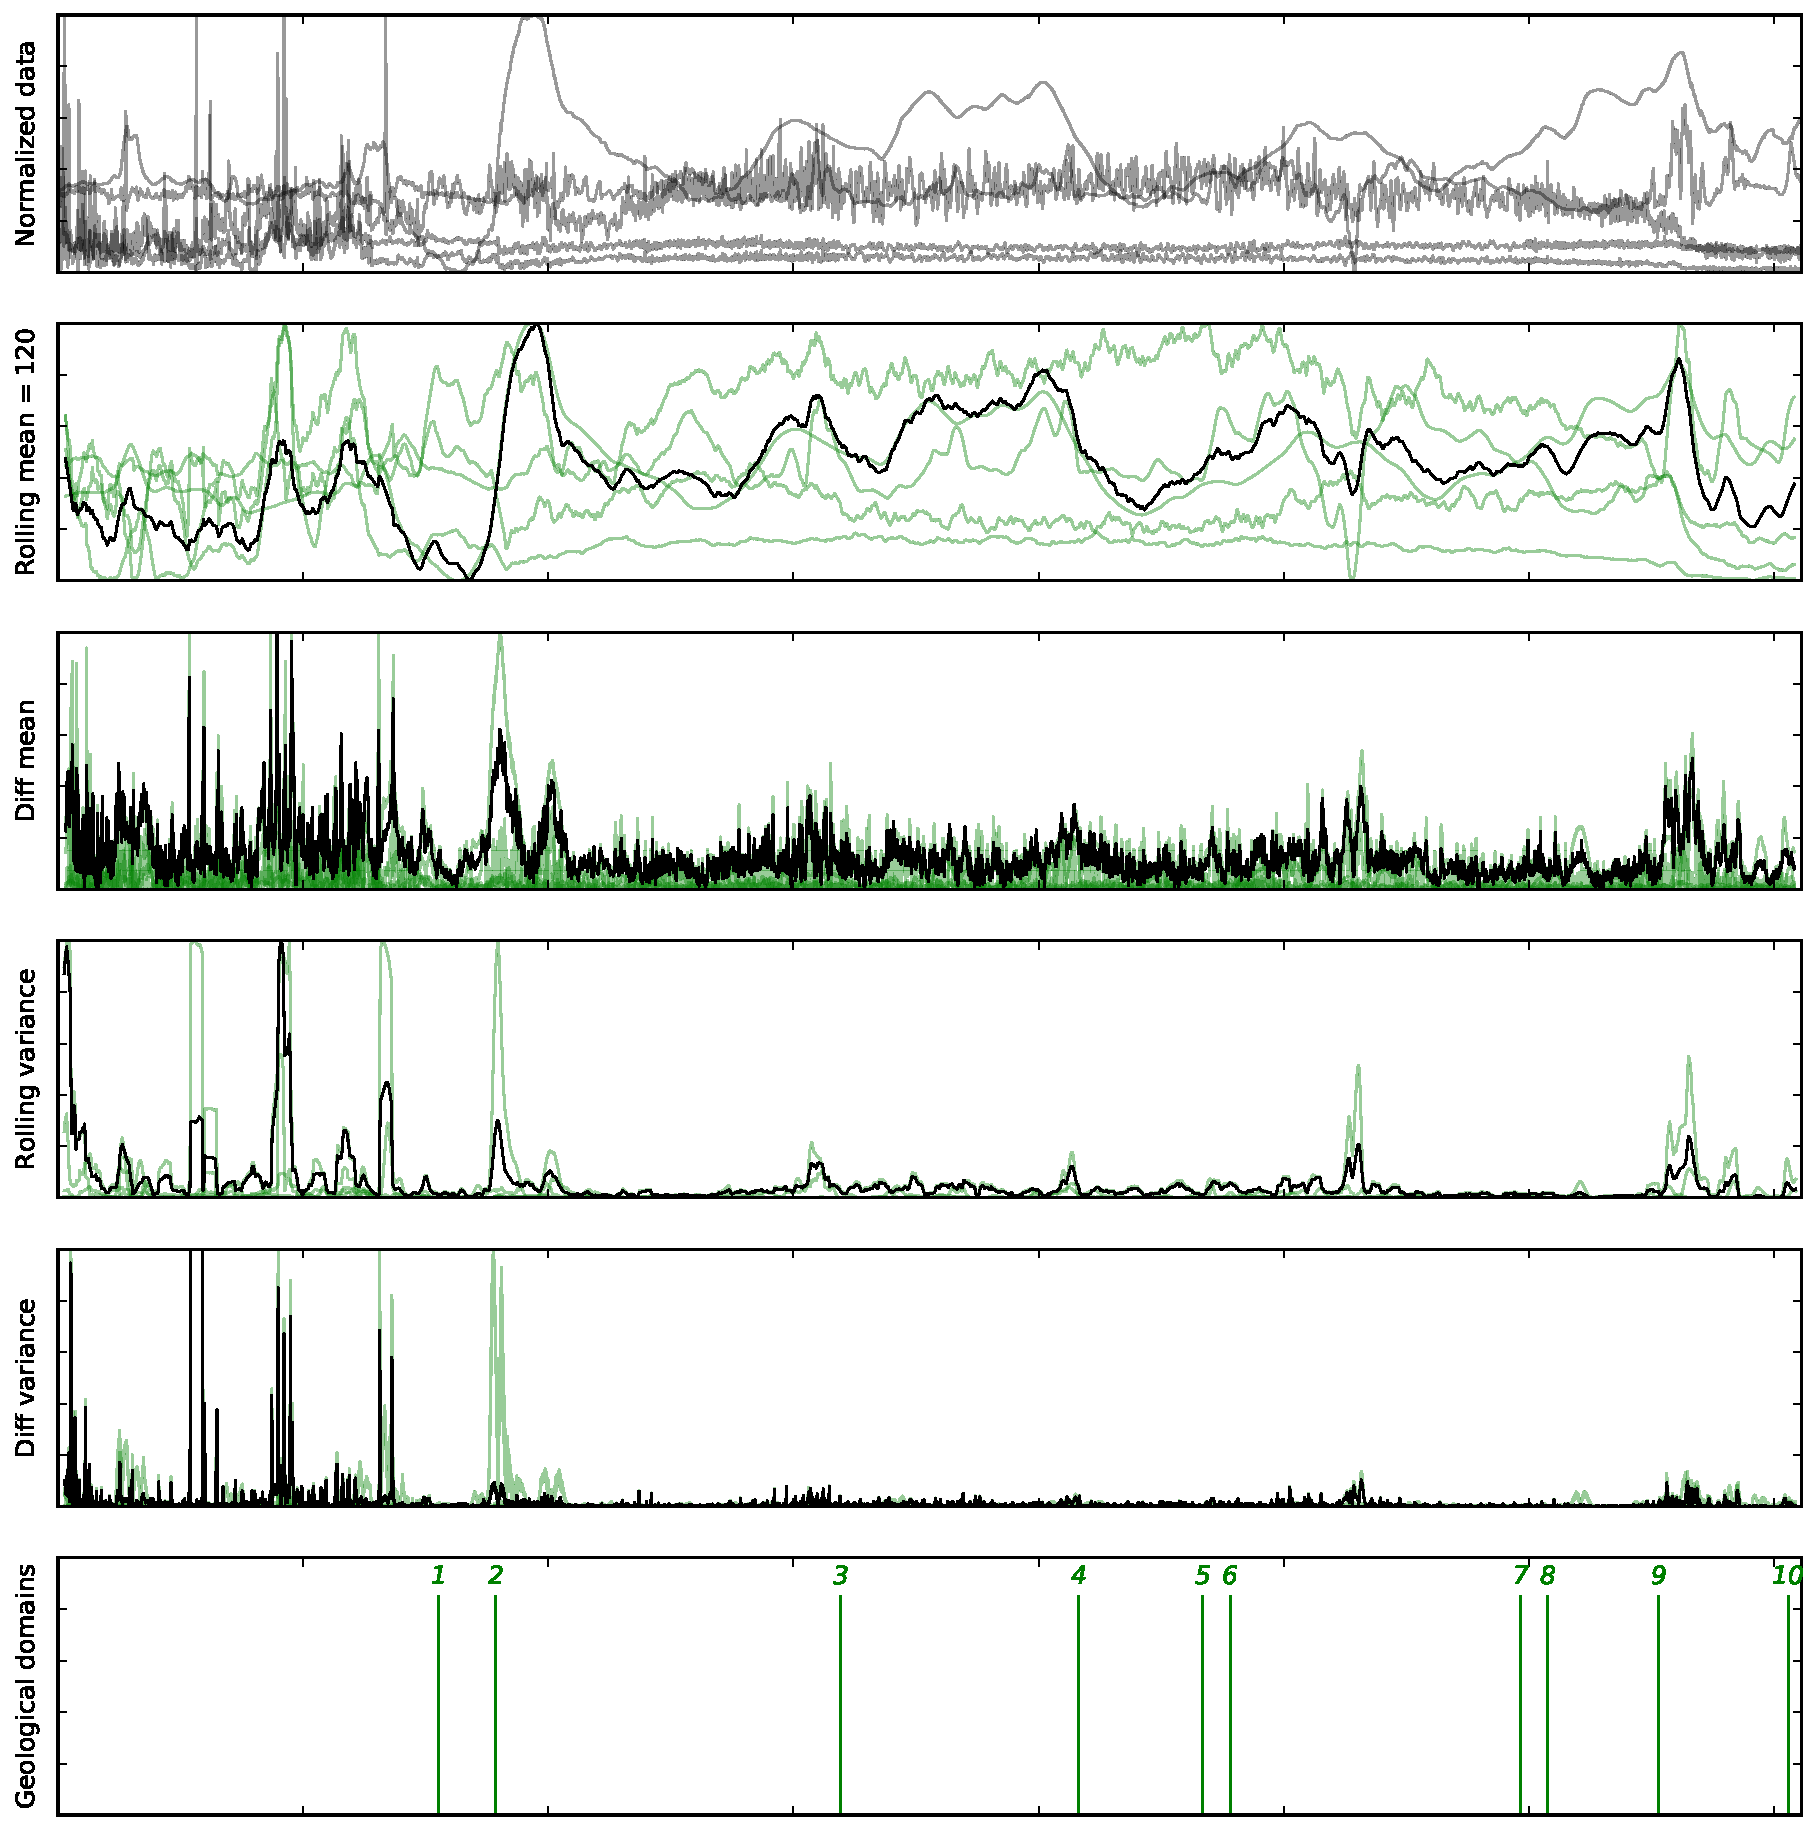
\includegraphics[width=1\linewidth]{../fig/naive_ga_vpt_line_16}
	\caption[Naïve 16]{Statistic analysis of Line 16. From left: 093 Yilgarn Craton (Super)-province (Block), 1: Mulga Rock (overprinted geophysical) zone; 093 Yilgarn (Super) province, 2: 003 Albany-Fraser Province, 3: Madura (250k map) region (or Naretha region); basement province, 4: Forrest (250k map) region, basement province, 5: Waigen (250k map) region; basement province, 6: Coompana Province (Block); basement province, 7: Cook (geophysically overprinted) zone (e.g., Cook 100k map); dolerite dyke swarm at northern edge of Coompana Block, basement unit (WT: Watson zone in version-1 map), 8: Christie structural subdomain (Barton 250k map); 036 Gawler Craton, 9: Fowler zone (Colona and Coorambie Fault zones), eastern Christie structural subdomain (NW Fowler 250k map); 036 Gawler Craton, 10: Wilgena and Nuyts structural subdomains; 036 Gawler Craton
}
	\label{fig:naive16}
\end{figure}

\begin{figure}[h]
\centering
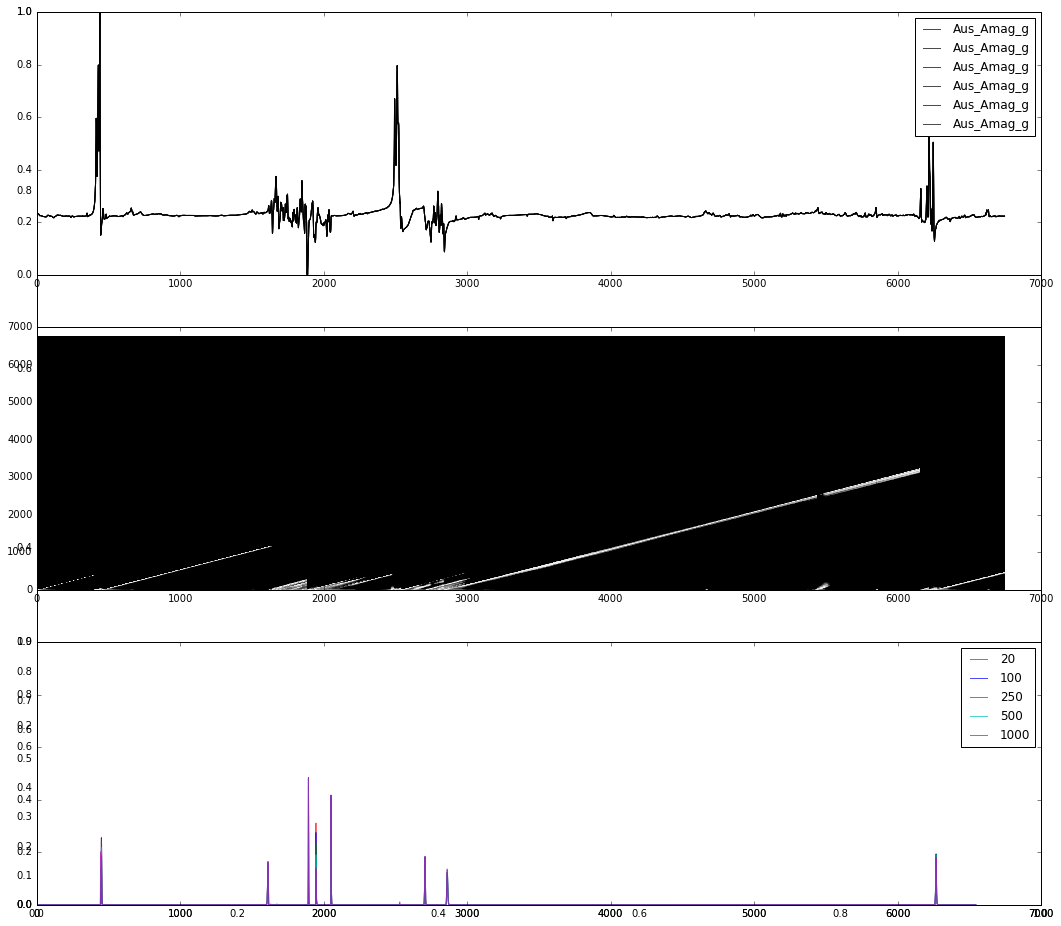
\includegraphics[width=1\linewidth]{../fig/1v_12_hi_Nw}
\caption[On-line changepoint detection. Line 12 (1:5)]{Online changepoint detection for Line 12. Upper plot shows all potential field data. Mid plot schow posterior probability based on magnetic data. A new run starts at each changepoint. Lower plot shows changepoint probability based on only magnetic data.}
\label{fig:1v12hinw}
\end{figure}

\begin{figure}
	\centering
	\begin{subfigure}[b]{1\textwidth}
		\centering
		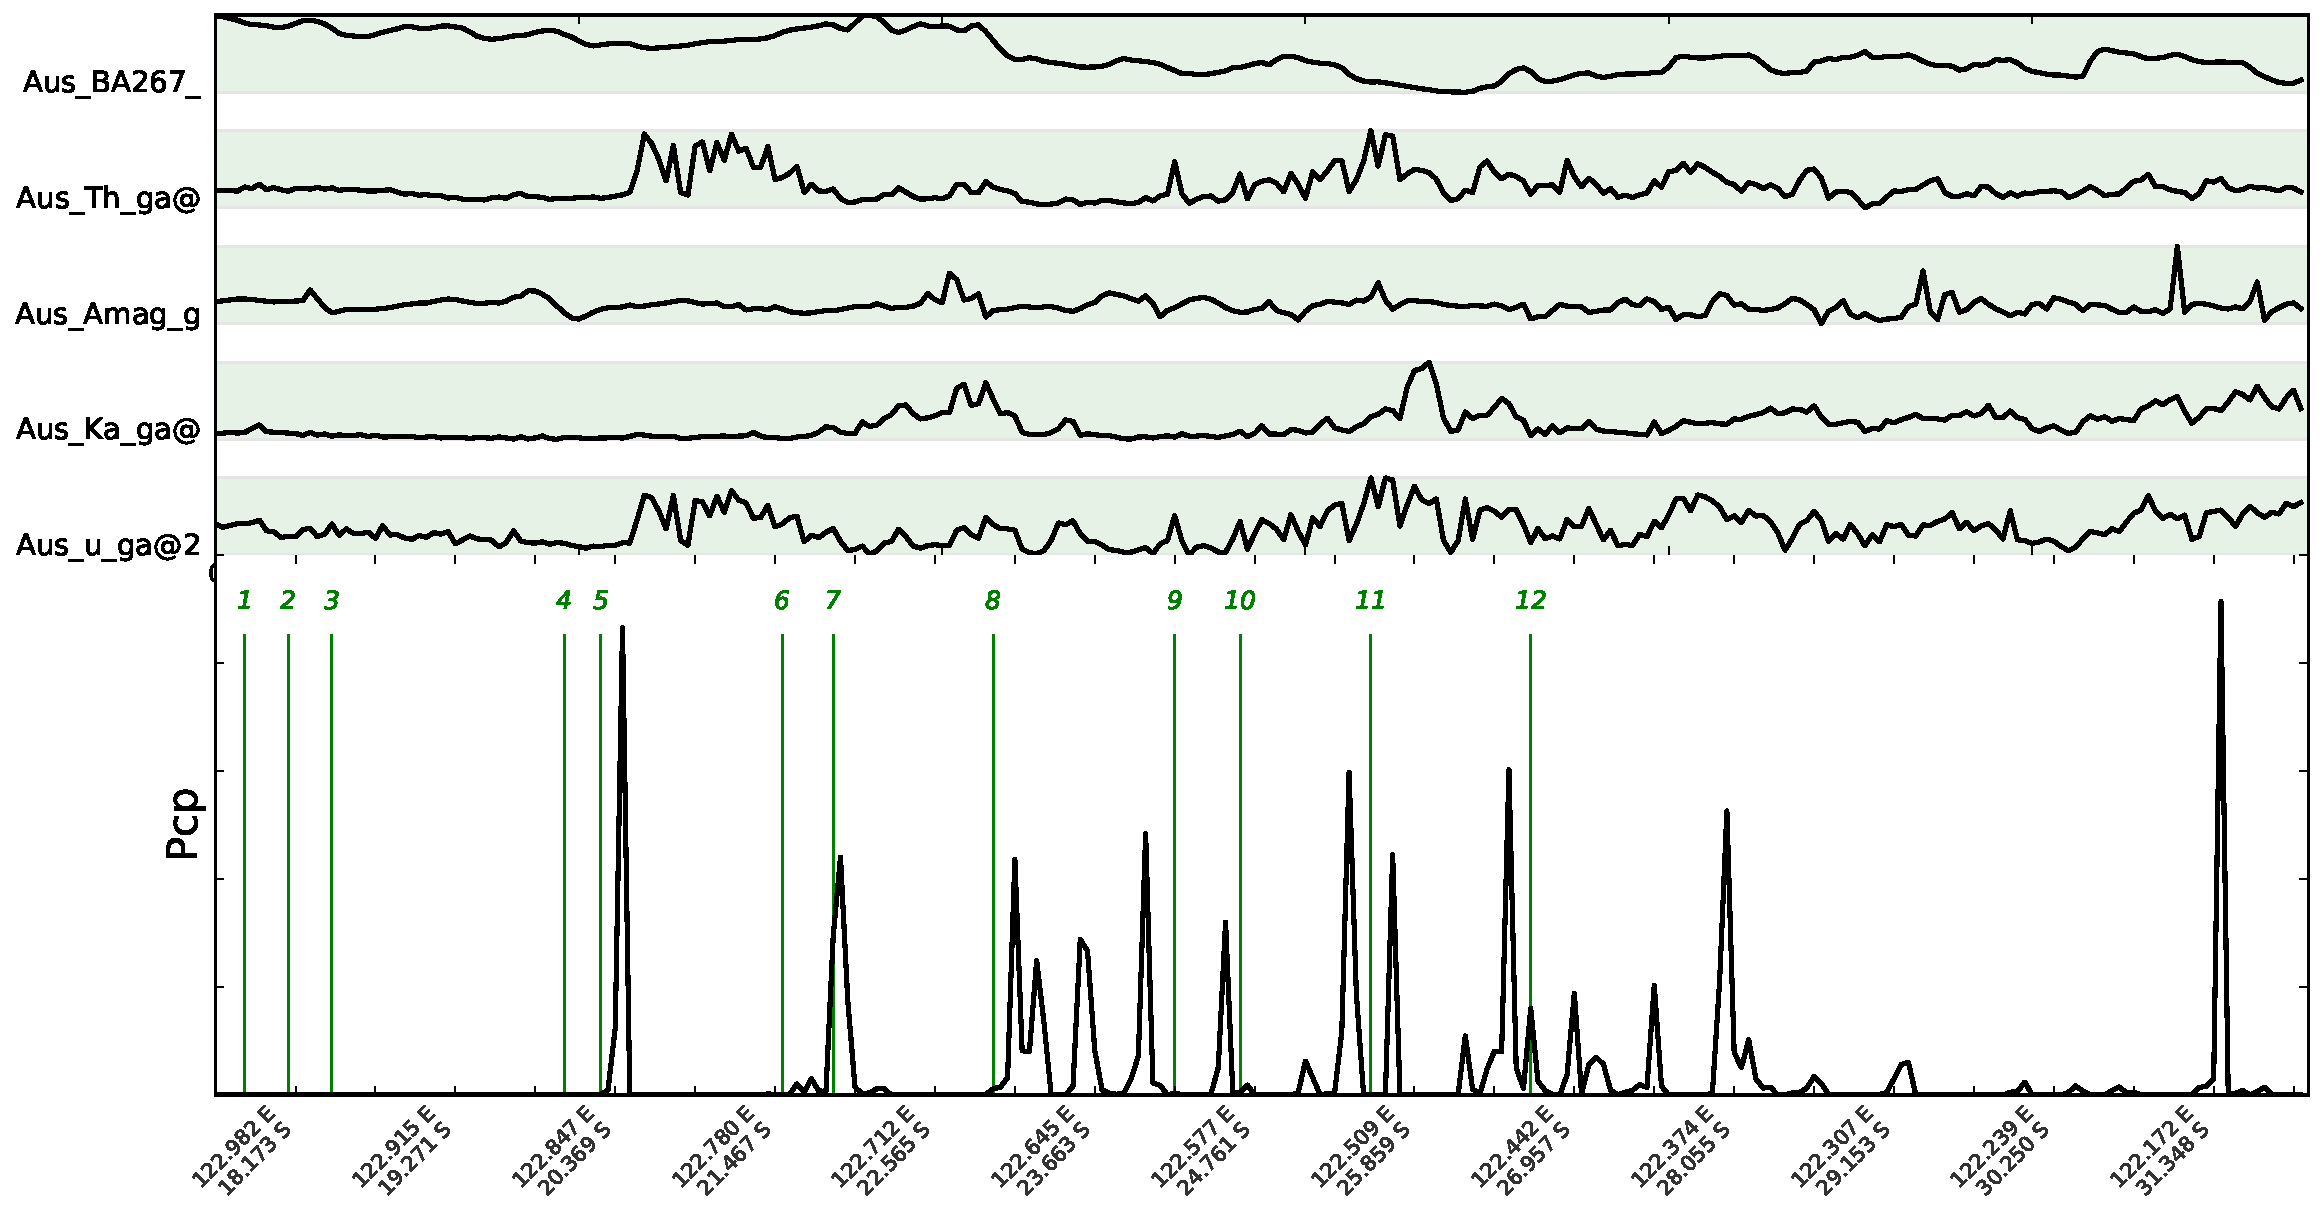
\includegraphics[width=0.9\linewidth]{../fig/ga_vpt_line_2}
		\caption[Line 2]{Line 2 subsampled 1:5 From left: Oscar Range region, basement province, 1: Nookanbah (250k) region, basement province, 2: Basement to Barbwire Terrace of 017 Canning Basin, 3: Lagrange (250k map) region, basement province, 4: Koop 100k map region (geophysicallly overprinted zone); basement province, 5: Roeves (gravity feature, Reeves Knoll) region; basement province, 6: 067 Paterson Province, 7: Rudall Inlier within  067 Paterson Province, 8: LD Lake Dissapointment  region (Gunanya 1:250k map); 067 Paterson Province (?), 9: Capricorn East (geophysical) region of Capricorn Orogen (e.g., Trainor 100k map); basement province (poorly defined), 10: Basement to 011 Bangemall Basin; Capricorn Orogen, 11: Overlies NE Yilgarn, 12: 093 Yilgarn Craton (Super)-province (Block)
}
		\label{fig:galine2}
	\end{subfigure}
	
	\begin{subfigure}[b]{1\textwidth}
		\centering
		\includegraphics[width=0.9\linewidth]{../fig/ga_vpt_line_2_lo}
		\caption[Line 2]{Line 2 subsampled 1:50 From left: Oscar Range region, basement province, 1: Nookanbah (250k) region, basement province, 2: Basement to Barbwire Terrace of 017 Canning Basin, 3: Lagrange (250k map) region, basement province, 4: Koop 100k map region (geophysicallly overprinted zone); basement province, 5: Roeves (gravity feature, Reeves Knoll) region; basement province, 6: 067 Paterson Province, 7: Rudall Inlier within  067 Paterson Province, 8: LD Lake Dissapointment  region (Gunanya 1:250k map); 067 Paterson Province (?), 9: Capricorn East (geophysical) region of Capricorn Orogen (e.g., Trainor 100k map); basement province (poorly defined), 10: Basement to 011 Bangemall Basin; Capricorn Orogen, 11: Overlies NE Yilgarn, 12: 093 Yilgarn Craton (Super)-province (Block)
}
		\label{fig:galine2_lo}
	\end{subfigure}
	
	\caption[Line 2]{Line 2}
\end{figure}

\begin{figure}
	\centering
	\begin{subfigure}[b]{1\textwidth}
		\centering
		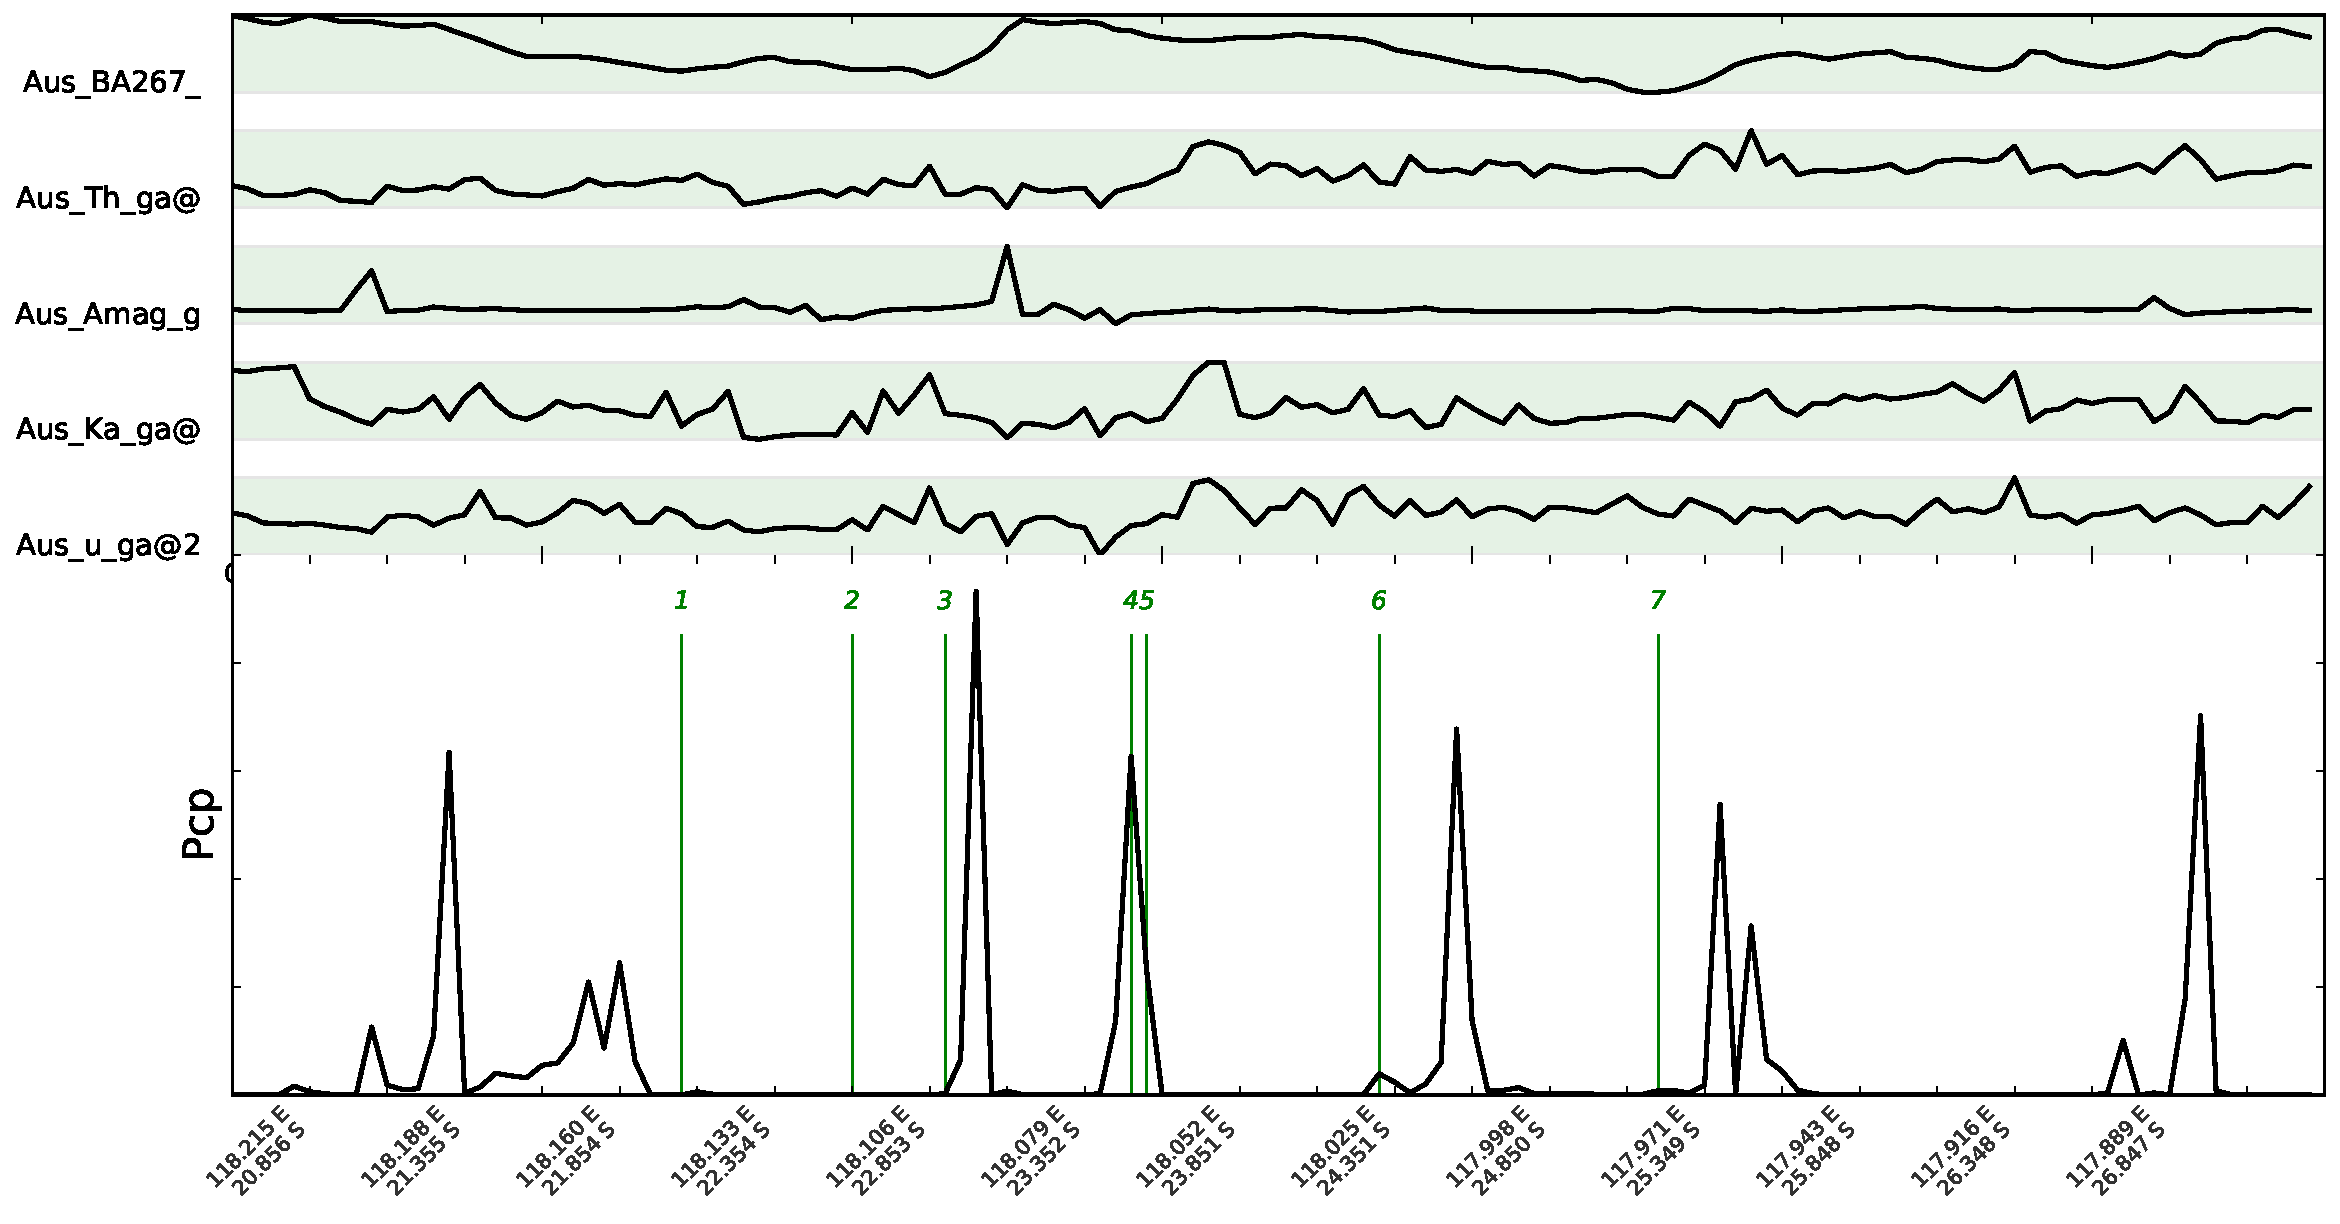
\includegraphics[width=0.9\linewidth]{../fig/ga_vpt_line_12}
		\caption[Line 12]{Line 12 subsampled 1:5 From left: 070 Pilbara Province (Craton/ Block), 1: 041 Hamersley Basin; overlies 070 Pilbara Craton, 2: 070 Pilbara Province (Craton/ Block), 3: 041 Hamersley Basin; overlies 070 Pilbara Craton, 4: 070 Pilbara Province (Craton/ Block), 5: Mount Vernon (100k map) region; 112 Asburton Basin; marginal to Capricorn Orogen, 6: Collier (250k map) region of Capricorn Orogen; southern 035 Gascoyne Province, 7: 093 Yilgarn Craton (Super)-province (Block)
}
		\label{fig:galine12}
	\end{subfigure}
	
	\begin{subfigure}[b]{1\textwidth}
		\centering
		\includegraphics[width=0.9\linewidth]{../fig/ga_vpt_line_12_lo}
		\caption[Line 12]{Line 12 subsampled 1:50 From left: 070 Pilbara Province (Craton/ Block), 1: 041 Hamersley Basin; overlies 070 Pilbara Craton, 2: 070 Pilbara Province (Craton/ Block), 3: 041 Hamersley Basin; overlies 070 Pilbara Craton, 4: 070 Pilbara Province (Craton/ Block), 5: Mount Vernon (100k map) region; 112 Asburton Basin; marginal to Capricorn Orogen, 6: Collier (250k map) region of Capricorn Orogen; southern 035 Gascoyne Province, 7: 093 Yilgarn Craton (Super)-province (Block)
}
		\label{fig:galine12_lo}
	\end{subfigure}
	
	\caption[Line 12]{Line 12}
\end{figure}

\begin{figure}
	\centering
	\begin{subfigure}[b]{1\textwidth}
		\centering
		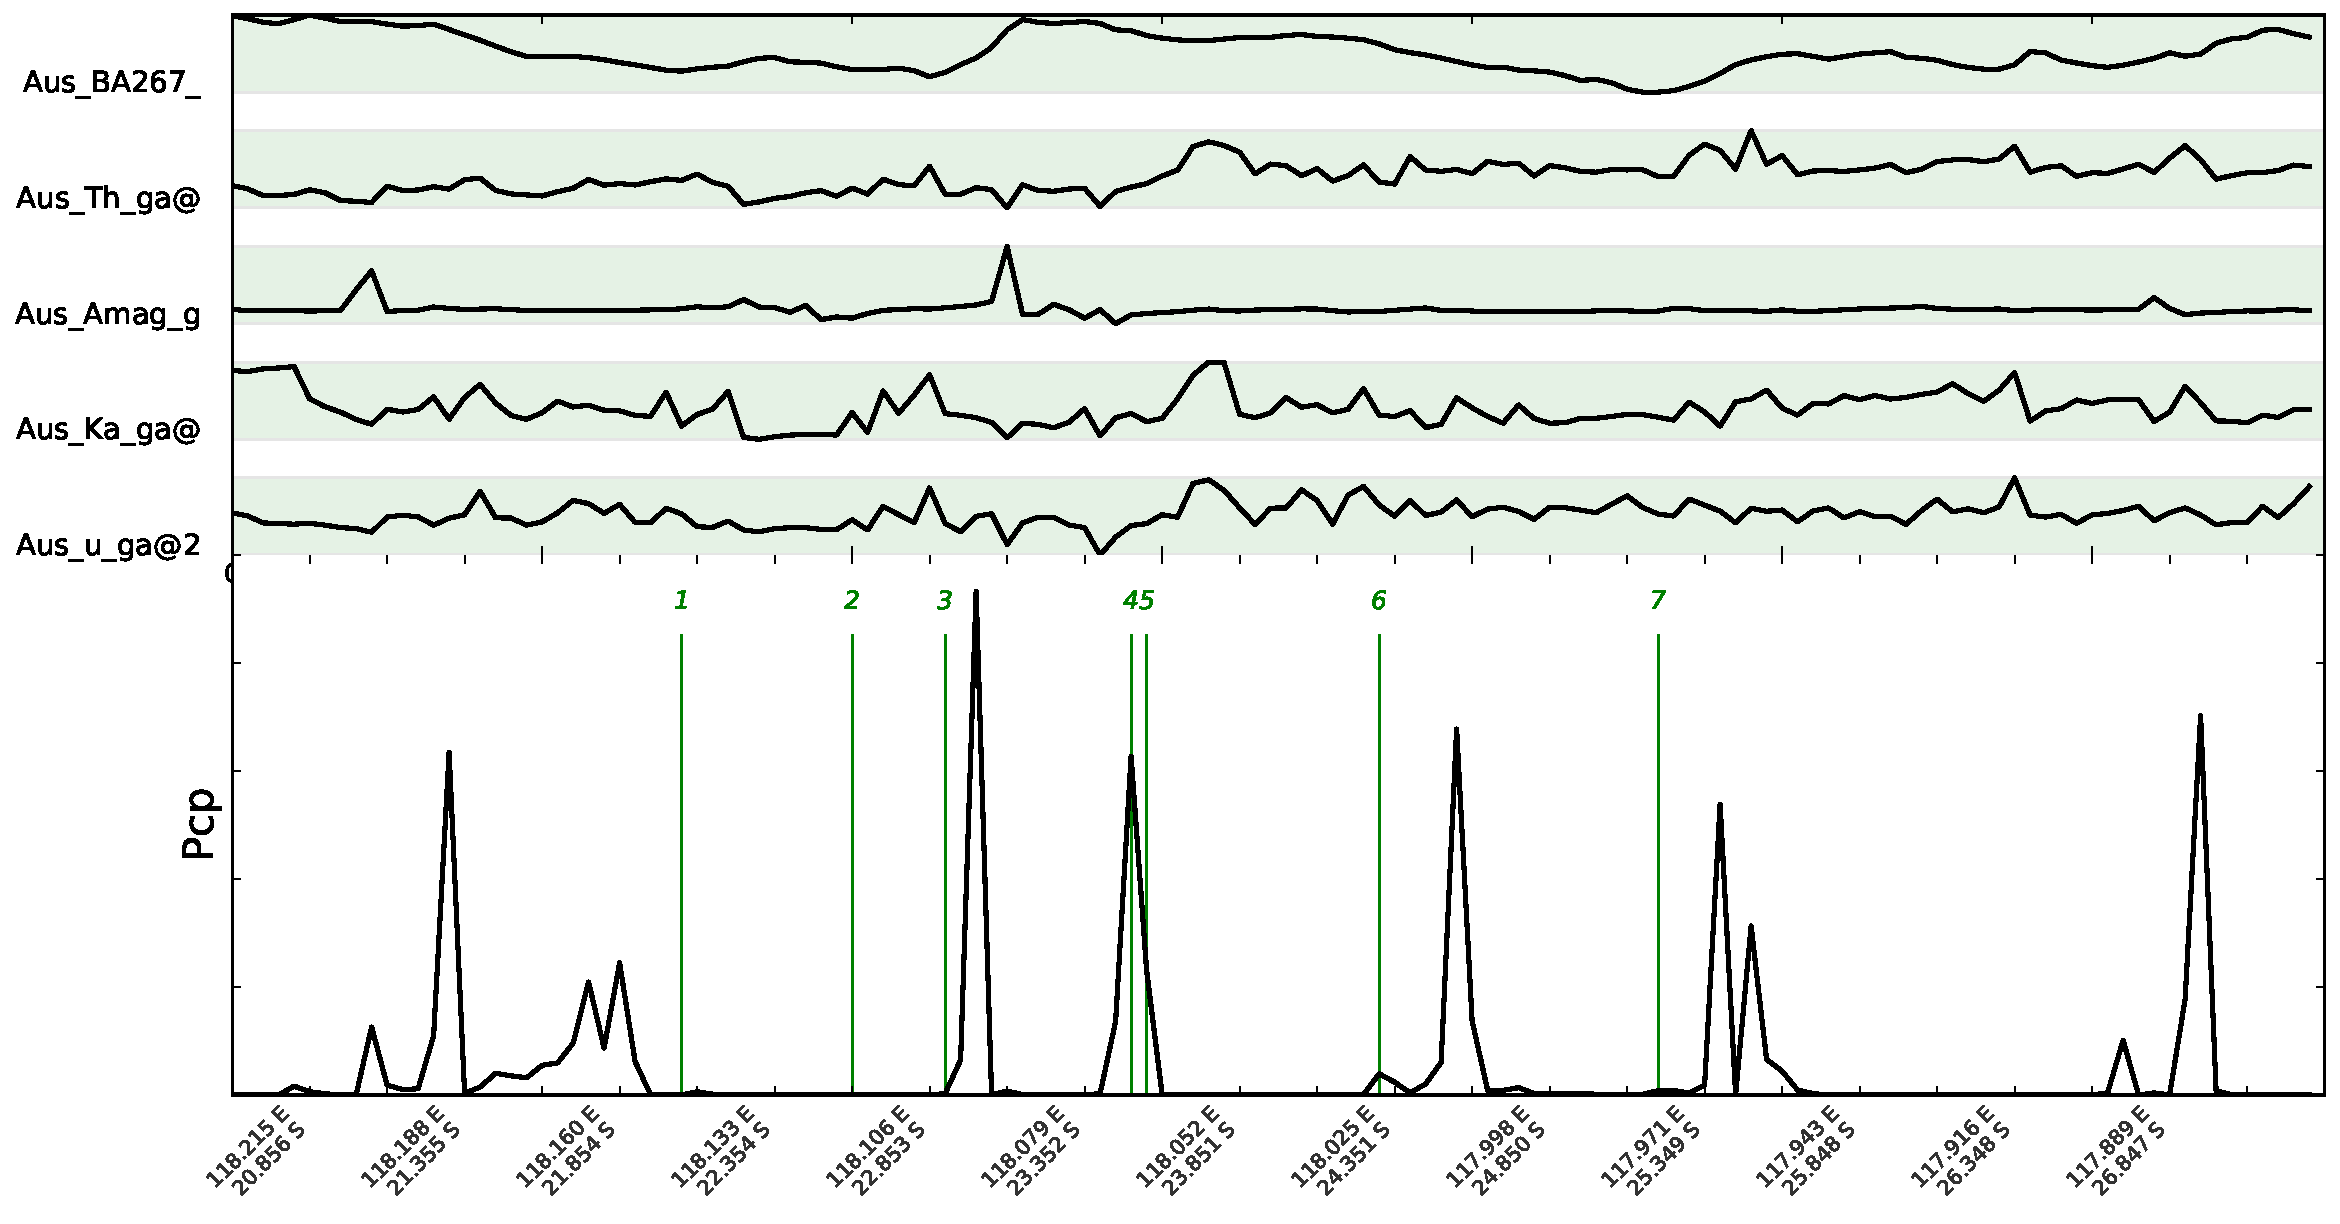
\includegraphics[width=0.9\linewidth]{../fig/ga_vpt_line_12}
		\caption[Line 12]{Line 12 subsampled 1:5 From left: 070 Pilbara Province (Craton/ Block), 1: 041 Hamersley Basin; overlies 070 Pilbara Craton, 2: 070 Pilbara Province (Craton/ Block), 3: 041 Hamersley Basin; overlies 070 Pilbara Craton, 4: 070 Pilbara Province (Craton/ Block), 5: Mount Vernon (100k map) region; 112 Asburton Basin; marginal to Capricorn Orogen, 6: Collier (250k map) region of Capricorn Orogen; southern 035 Gascoyne Province, 7: 093 Yilgarn Craton (Super)-province (Block)
}
		\label{fig:galine12}
	\end{subfigure}
	
	\begin{subfigure}[b]{1\textwidth}
		\centering
		\includegraphics[width=0.9\linewidth]{../fig/ga_vpt_line_12_lo}
		\caption[Line 12]{Line 12 subsampled 1:50 From left: 070 Pilbara Province (Craton/ Block), 1: 041 Hamersley Basin; overlies 070 Pilbara Craton, 2: 070 Pilbara Province (Craton/ Block), 3: 041 Hamersley Basin; overlies 070 Pilbara Craton, 4: 070 Pilbara Province (Craton/ Block), 5: Mount Vernon (100k map) region; 112 Asburton Basin; marginal to Capricorn Orogen, 6: Collier (250k map) region of Capricorn Orogen; southern 035 Gascoyne Province, 7: 093 Yilgarn Craton (Super)-province (Block)
}
		\label{fig:galine12_lo}
	\end{subfigure}
	
	\caption[Line 12]{Line 12}
\end{figure}

\begin{figure}
	\centering
	\begin{subfigure}[b]{1\textwidth}
		\centering
		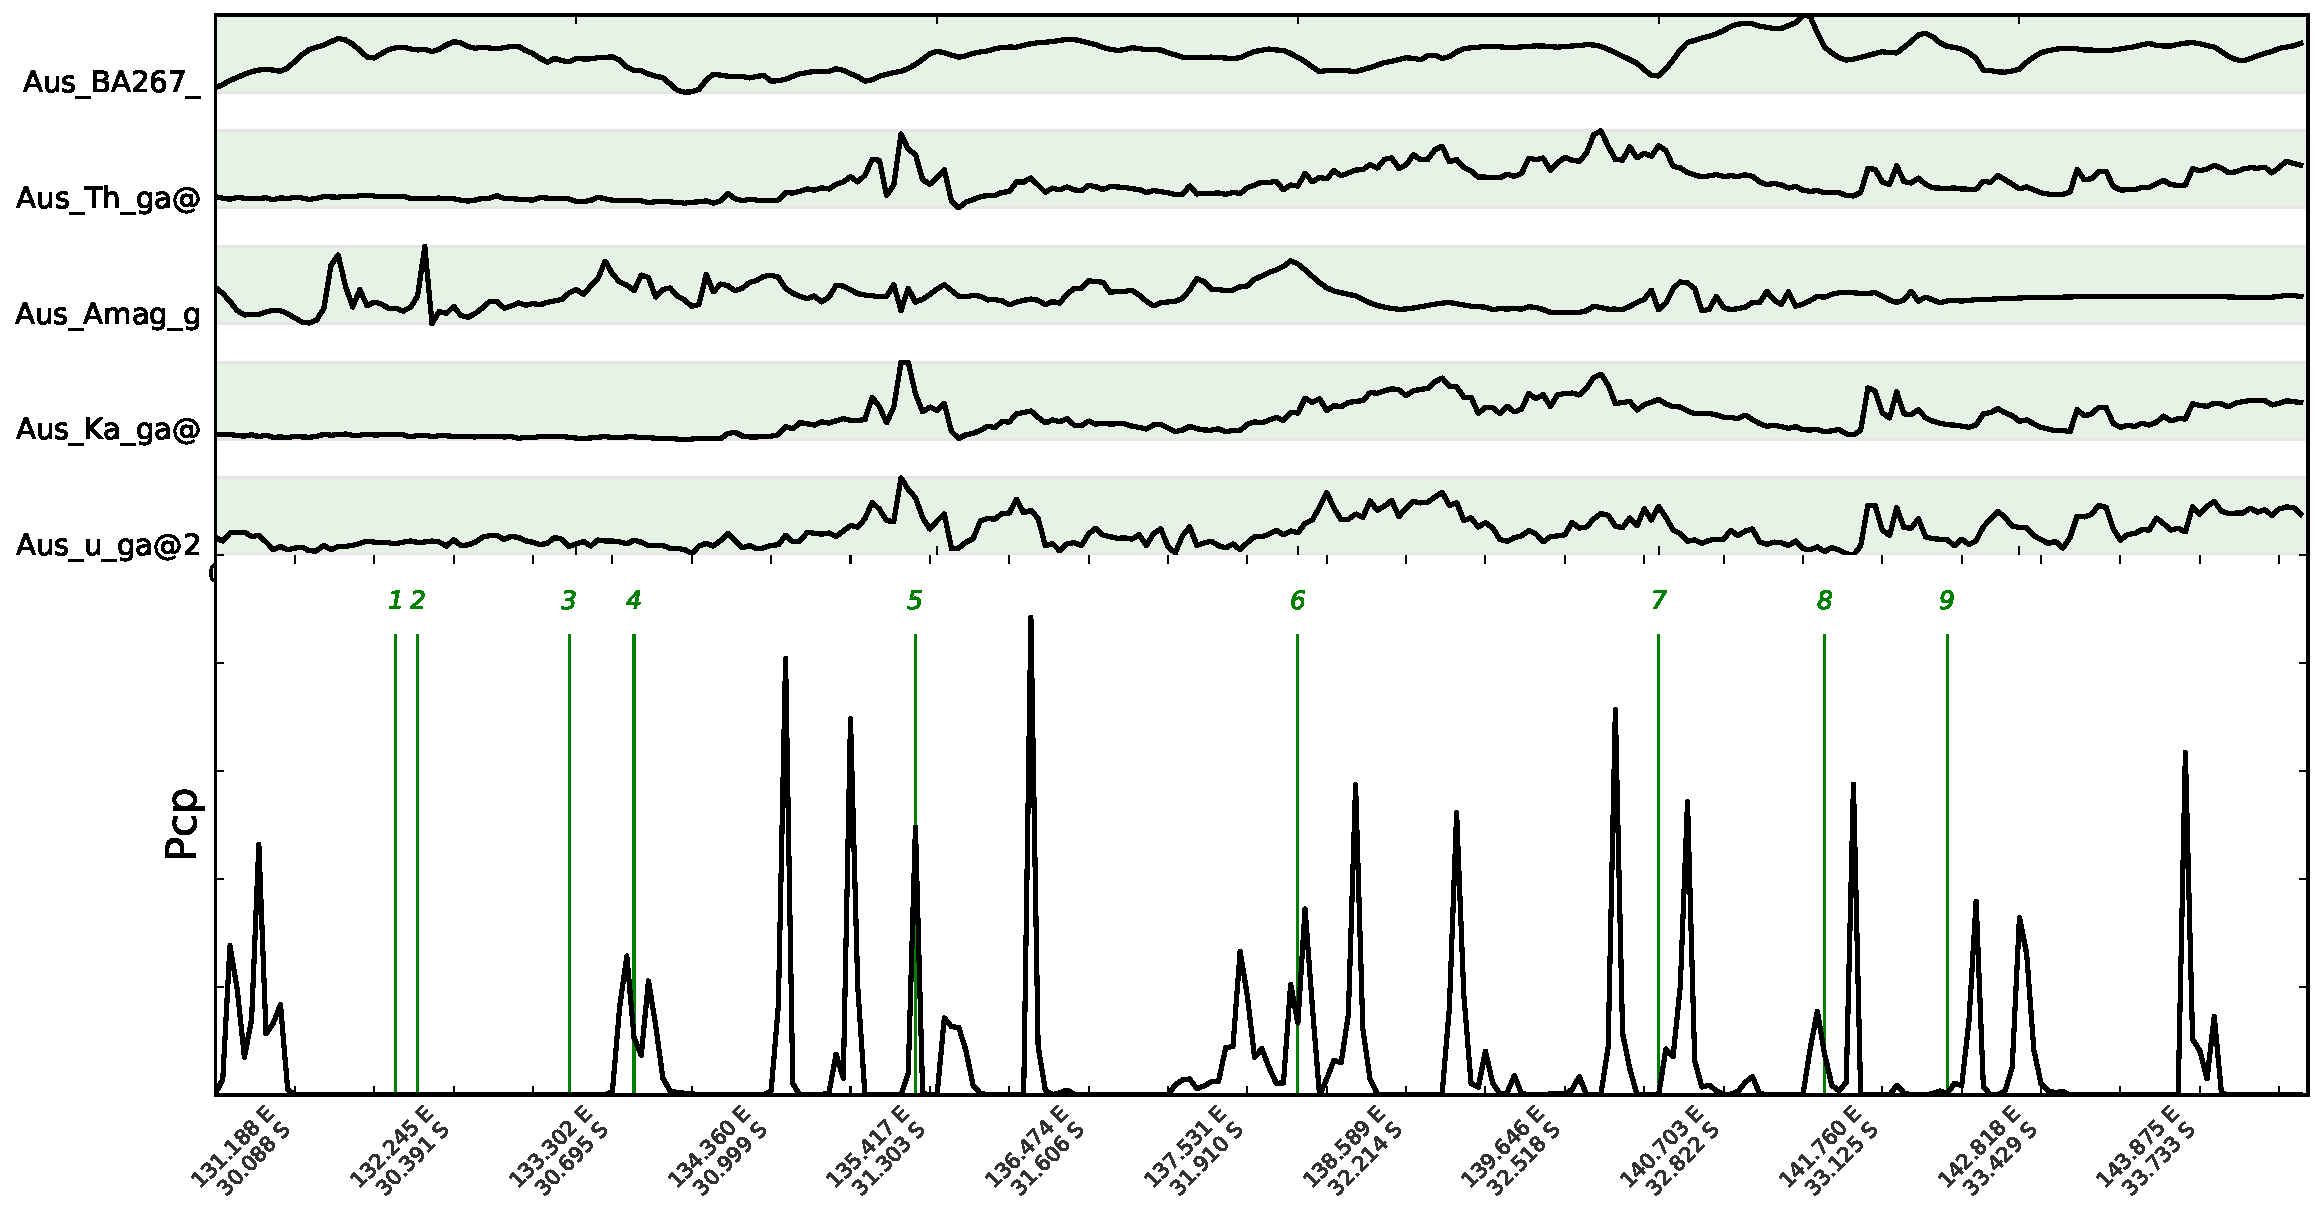
\includegraphics[width=0.9\linewidth]{../fig/ga_vpt_line_14}
		\caption[Line 14]{Line 14 subsampled 1:5 From left: Nawa structural subdomain, basement province (includes Ammaroodina Inlier); in old 036 {superseded} Gawler Craton, 1: Karari Fault Zone; N-margin to 036 Gawler Craton (redefined craton margin), 2: Christie structural subdomain (Barton 250k map); 036 Gawler Craton, 3: Fowler zone (Colona and Coorambie Fault zones), eastern Christie structural subdomain (NW Fowler 250k map); 036 Gawler Craton, 4: Wilgena and Nuyts structural subdomains; 036 Gawler Craton, 5: Gawler Range Volcanic Subprovince (geophysical subdivision); 036 Gawler Craton, 6: 002 Adelaide Province (Fold Belt), 7: 044 Kanmantoo Province (Fold Belt), 8: Glenelg and Stavely Zones; western margin of 047 Lachlan, 9: Western part of 047 Lachlan Province (Fold Belt)
}
		\label{fig:galine14}
	\end{subfigure}
	
	\begin{subfigure}[b]{1\textwidth}
		\centering
		\includegraphics[width=0.9\linewidth]{../fig/ga_vpt_line_14_lo}
		\caption[Line 14]{Line 14 subsampled 1:50 From left: Nawa structural subdomain, basement province (includes Ammaroodina Inlier); in old 036 {superseded} Gawler Craton, 1: Karari Fault Zone; N-margin to 036 Gawler Craton (redefined craton margin), 2: Christie structural subdomain (Barton 250k map); 036 Gawler Craton, 3: Fowler zone (Colona and Coorambie Fault zones), eastern Christie structural subdomain (NW Fowler 250k map); 036 Gawler Craton, 4: Wilgena and Nuyts structural subdomains; 036 Gawler Craton, 5: Gawler Range Volcanic Subprovince (geophysical subdivision); 036 Gawler Craton, 6: 002 Adelaide Province (Fold Belt), 7: 044 Kanmantoo Province (Fold Belt), 8: Glenelg and Stavely Zones; western margin of 047 Lachlan, 9: Western part of 047 Lachlan Province (Fold Belt)
}
		\label{fig:galine14_lo}
	\end{subfigure}
	
	\caption[Line 14]{Line 14}
\end{figure}

\begin{figure}
	\centering
	\begin{subfigure}[b]{1\textwidth}
		\centering
		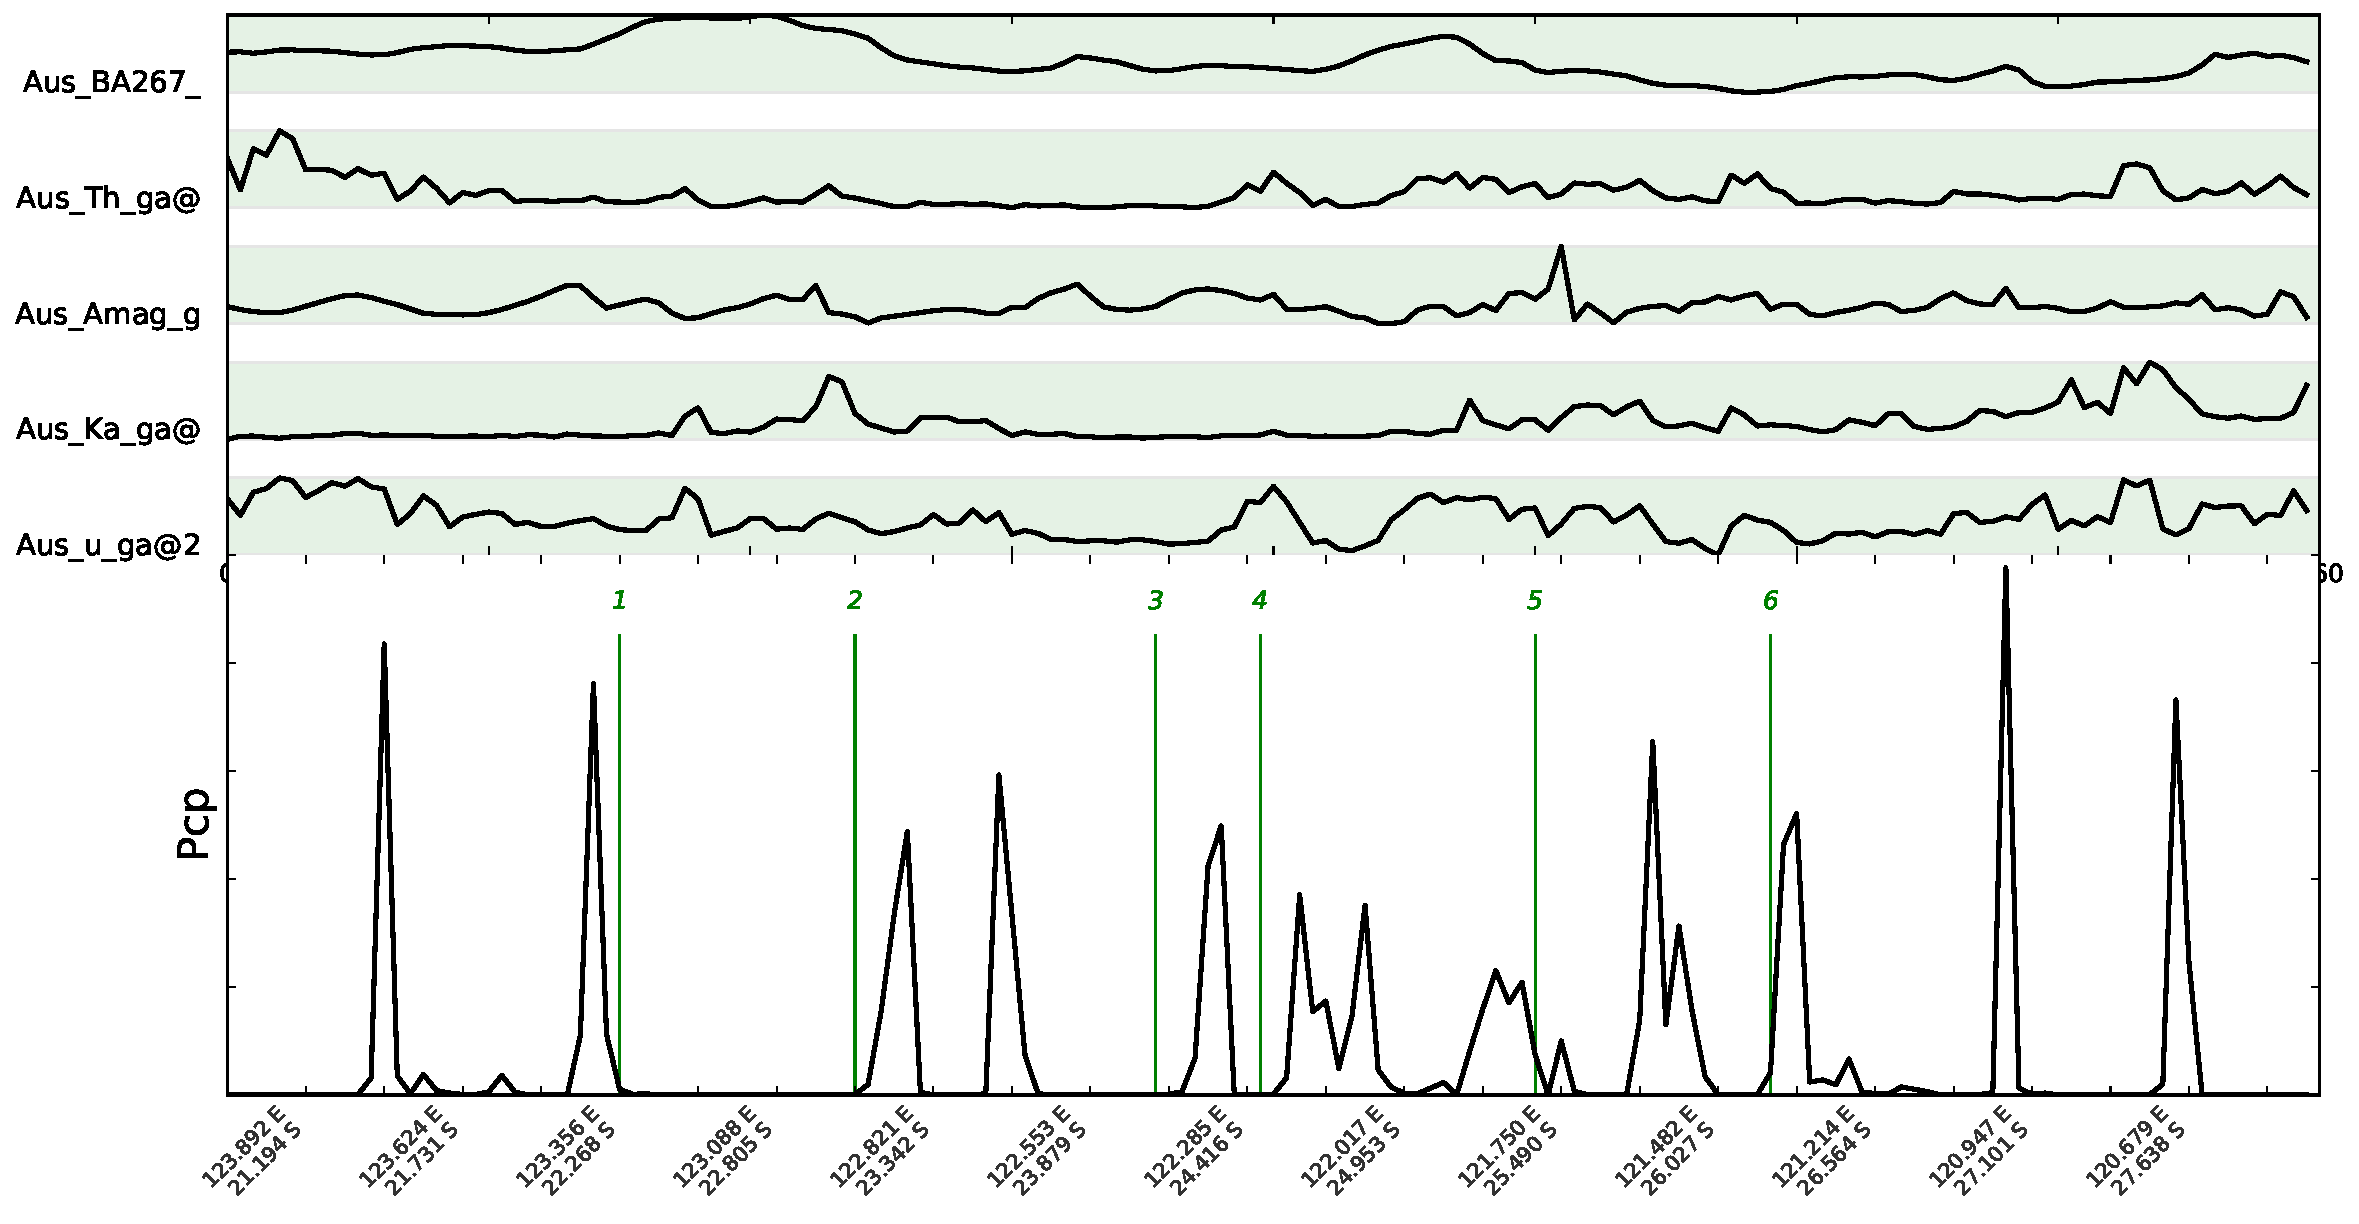
\includegraphics[width=0.9\linewidth]{../fig/ga_vpt_line_15}
		\caption[Line 15]{Line 15 subsampled 1:5 From left: Roeves (gravity feature, Reeves Knoll) region; basement province, 1: Rudall Inlier within  067 Paterson Province, 2: LD Lake Dissapointment  region (Gunanya 1:250k map); 067 Paterson Province (?), 3: Capricorn East (geophysical) region of Capricorn Orogen (e.g., Trainor 100k map); basement province (poorly defined), 4: Basement to 011 Bangemall Basin; Capricorn Orogen, 5: Overlies NE Yilgarn, 6: 093 Yilgarn Craton (Super)-province (Block)
}
		\label{fig:galine15}
	\end{subfigure}
	
	\begin{subfigure}[b]{1\textwidth}
		\centering
		\includegraphics[width=0.9\linewidth]{../fig/ga_vpt_line_15_lo}
		\caption[Line 15]{Line 15 subsampled 1:50 From left: Roeves (gravity feature, Reeves Knoll) region; basement province, 1: Rudall Inlier within  067 Paterson Province, 2: LD Lake Dissapointment  region (Gunanya 1:250k map); 067 Paterson Province (?), 3: Capricorn East (geophysical) region of Capricorn Orogen (e.g., Trainor 100k map); basement province (poorly defined), 4: Basement to 011 Bangemall Basin; Capricorn Orogen, 5: Overlies NE Yilgarn, 6: 093 Yilgarn Craton (Super)-province (Block)
}
		\label{fig:galine15_lo}
	\end{subfigure}
	
	\caption[Line 15]{Line 15}
\end{figure}

\begin{figure}
	\centering
	\begin{subfigure}[b]{1\textwidth}
	\centering
	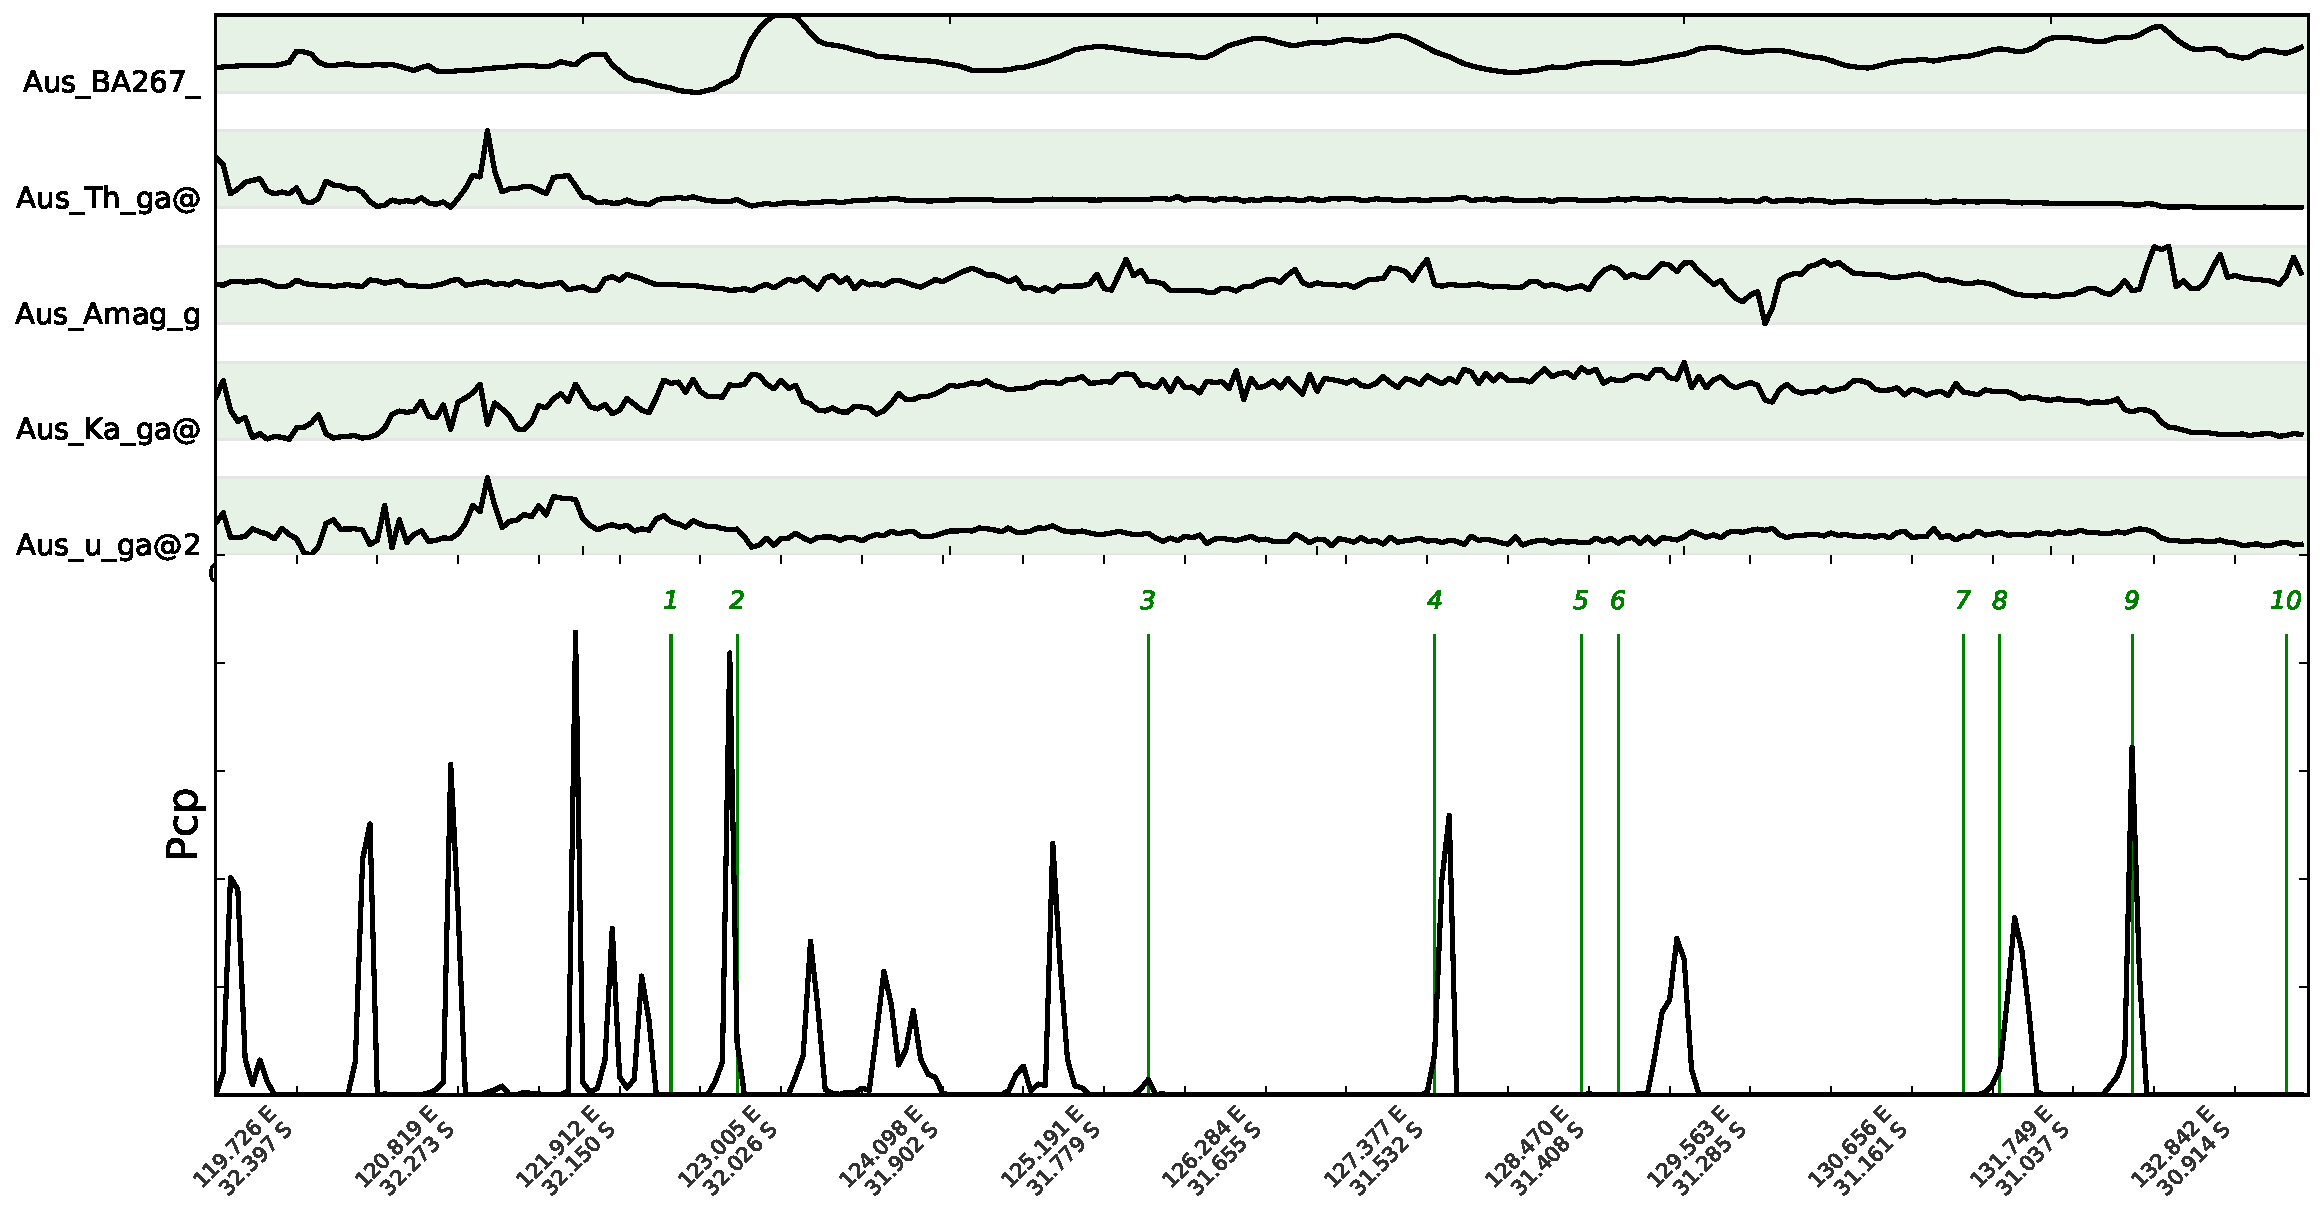
\includegraphics[width=0.9\linewidth]{../fig/ga_vpt_line_16}
	\caption[Line 16]{Line 15 subsampled 1:5 From left: 093 Yilgarn Craton (Super)-province (Block), 1: Mulga Rock (overprinted geophysical) zone; 093 Yilgarn (Super) province, 2: 003 Albany-Fraser Province, 3: Madura (250k map) region (or Naretha region); basement province, 4: Forrest (250k map) region, basement province, 5: Waigen (250k map) region; basement province, 6: Coompana Province (Block); basement province, 7: Cook (geophysically overprinted) zone (e.g., Cook 100k map); dolerite dyke swarm at northern edge of Coompana Block, basement unit (WT: Watson zone in version-1 map), 8: Christie structural subdomain (Barton 250k map); 036 Gawler Craton, 9: Fowler zone (Colona and Coorambie Fault zones), eastern Christie structural subdomain (NW Fowler 250k map); 036 Gawler Craton, 10: Wilgena and Nuyts structural subdomains; 036 Gawler Craton
}
	\label{fig:galine16}
	\end{subfigure}
	
	\begin{subfigure}[b]{1\textwidth}
	\centering
	\includegraphics[width=0.9\linewidth]{../fig/ga_vpt_line_16_lo}
	\caption[Line 16]{Line 16 subsampled 1:50 From left: 093 Yilgarn Craton (Super)-province (Block), 1: Mulga Rock (overprinted geophysical) zone; 093 Yilgarn (Super) province, 2: 003 Albany-Fraser Province, 3: Madura (250k map) region (or Naretha region); basement province, 4: Forrest (250k map) region, basement province, 5: Waigen (250k map) region; basement province, 6: Coompana Province (Block); basement province, 7: Cook (geophysically overprinted) zone (e.g., Cook 100k map); dolerite dyke swarm at northern edge of Coompana Block, basement unit (WT: Watson zone in version-1 map), 8: Christie structural subdomain (Barton 250k map); 036 Gawler Craton, 9: Fowler zone (Colona and Coorambie Fault zones), eastern Christie structural subdomain (NW Fowler 250k map); 036 Gawler Craton, 10: Wilgena and Nuyts structural subdomains; 036 Gawler Craton
}
	\label{fig:galine16_lo}
	\end{subfigure}
	
	\caption[Line 16]{Line 16}
\end{figure}

\begin{figure}
	\centering
	\begin{subfigure}[b]{1\textwidth}
		\centering
		\includegraphics[width=0.65\linewidth]{../fig/no_radio_ga_vpt_line_2}
		\caption[Line 2, no radometry]{Line 2 without radiometric data. Subsampled 1:5 From left: Oscar Range region, basement province, 1: Nookanbah (250k) region, basement province, 2: Basement to Barbwire Terrace of 017 Canning Basin, 3: Lagrange (250k map) region, basement province, 4: Koop 100k map region (geophysicallly overprinted zone); basement province, 5: Roeves (gravity feature, Reeves Knoll) region; basement province, 6: 067 Paterson Province, 7: Rudall Inlier within  067 Paterson Province, 8: LD Lake Dissapointment  region (Gunanya 1:250k map); 067 Paterson Province (?), 9: Capricorn East (geophysical) region of Capricorn Orogen (e.g., Trainor 100k map); basement province (poorly defined), 10: Basement to 011 Bangemall Basin; Capricorn Orogen, 11: Overlies NE Yilgarn, 12: 093 Yilgarn Craton (Super)-province (Block)
}
	\label{fig:galine2_no}
\end{subfigure}
	
	\begin{subfigure}[b]{1\textwidth}
		\centering
		\includegraphics[width=0.65\linewidth]{../fig/no_radio_ga_vpt_line_12}
		\caption[Line 12, no radometry]{Line 12 without radiometric data. Subsampled 1:5. From left: 070 Pilbara Province (Craton/ Block), 1: 041 Hamersley Basin; overlies 070 Pilbara Craton, 2: 070 Pilbara Province (Craton/ Block), 3: 041 Hamersley Basin; overlies 070 Pilbara Craton, 4: 070 Pilbara Province (Craton/ Block), 5: Mount Vernon (100k map) region; 112 Asburton Basin; marginal to Capricorn Orogen, 6: Collier (250k map) region of Capricorn Orogen; southern 035 Gascoyne Province, 7: 093 Yilgarn Craton (Super)-province (Block)
}
	\label{fig:galine12_no}
\end{subfigure}
	
	\begin{subfigure}[b]{1\textwidth}
			\centering
			\includegraphics[width=0.65\linewidth]{../fig/no_radio_ga_vpt_line_15}
			\caption[Line 15, no radometry]{Line 15 without radiometric data. Subsampled 1:5. From left: Roeves (gravity feature, Reeves Knoll) region; basement province, 1: Rudall Inlier within  067 Paterson Province, 2: LD Lake Dissapointment  region (Gunanya 1:250k map); 067 Paterson Province (?), 3: Capricorn East (geophysical) region of Capricorn Orogen (e.g., Trainor 100k map); basement province (poorly defined), 4: Basement to 011 Bangemall Basin; Capricorn Orogen, 5: Overlies NE Yilgarn, 6: 093 Yilgarn Craton (Super)-province (Block)
}
			\label{fig:galine15_no}
\end{subfigure}
		
	\caption[Line 2, 12 and 15 without radometry]{Lines 2, 12 and 15. Off-line changepoint detection without use of radiometric data. Sub-sampled 1:5.}
\end{figure}

\begin{figure}
	\centering
	\begin{subfigure}[b]{1\textwidth}
		\centering
		\includegraphics[width=0.7\linewidth]{../fig/no_radio_ga_vpt_line_13}
		\caption[Line 13, no radometry]{Line 13 without radiometric data. Subsampled 1:5. From left: Waigen (250k map) region; basement province, 1: Nawa structural subdomain, basement province (includes Ammaroodina Inlier); in old 036 {superseded} Gawler Craton, 2: Western magnetic part of Mabel Creek (100k map) region (geophysical subdivision); in old 036 (superseded) Gawler Craton, 3: Karari Fault Zone; N-margin to 036 Gawler Craton (redefined craton margin), 4: Christie structural subdomain (Barton 250k map); 036 Gawler Craton, 5: Challenger (Mine) region (Coober Pedy 250k map); 036 Gawler Craton, 6: Fowler zone (Colona and Coorambie Fault zones), eastern Christie structural subdomain (NW Fowler 250k map); 036 Gawler Craton, 7: Wilgena and Nuyts structural subdomains; 036 Gawler Craton, 8: Gawler Range Volcanic Subprovince (geophysical subdivision); 036 Gawler Craton, 9: 002 Adelaide Province (Fold Belt), 10: Curnamona craton (nucleus), basement province (includes Benagerie Ridge), 11: 108 Willyama subprovince (Block) and Olary subprovince (Willyama Inliers in South Australia) adjoining southern Curnamona (geological) craton (nucleus); 016 Broken Hill Province (Block), 12: Covered Willyama Province; 016 Broken Hill Block, 13: 108 Willyama subprovince (Block) and Olary subprovince (Willyama Inliers in South Australia) adjoining southern Curnamona (geological) craton (nucleus); 016 Broken Hill Province (Block), 14: Redan (geophysical overprinting) Zone; southern margin of 016 Broken Hill Province (Block), 15: 044 Kanmantoo Province (Fold Belt), 16: Glenelg and Stavely Zones; western margin of 047 Lachlan, 17: Western part of 047 Lachlan Province (Fold Belt)
}
	\label{fig:galine13_no}
\end{subfigure}

\begin{subfigure}[b]{1\textwidth}
	\centering
	\includegraphics[width=0.7\linewidth]{../fig/no_radio_ga_vpt_line_14}
	\caption[Line 14, without radiometry]{Line 14 without radiometric data. Sub-sampled 1:5. From left: Nawa structural subdomain, basement province (includes Ammaroodina Inlier); in old 036 {superseded} Gawler Craton, 1: Karari Fault Zone; N-margin to 036 Gawler Craton (redefined craton margin), 2: Christie structural subdomain (Barton 250k map); 036 Gawler Craton, 3: Fowler zone (Colona and Coorambie Fault zones), eastern Christie structural subdomain (NW Fowler 250k map); 036 Gawler Craton, 4: Wilgena and Nuyts structural subdomains; 036 Gawler Craton, 5: Gawler Range Volcanic Subprovince (geophysical subdivision); 036 Gawler Craton, 6: 002 Adelaide Province (Fold Belt), 7: 044 Kanmantoo Province (Fold Belt), 8: Glenelg and Stavely Zones; western margin of 047 Lachlan, 9: Western part of 047 Lachlan Province (Fold Belt)
}
\label{fig:galine14_no}
\end{subfigure}

\caption[Line 13 and 14 without radiometry]{Lines 13 and 14. Off-line changepoint detection without use of radiometric data. Sub-sampled 1:5.}
\end{figure}

\begin{figure}
	\centering
	\begin{subfigure}[b]{1\textwidth}
		\centering
		\includegraphics[width=0.7\linewidth]{../fig/no_radio_ga_vpt_line_16}
		\caption[Line 16, no radiometry]{Line 16 without radiometric data. Sub-sampled 1:5.} 
		\label{fig:galine16_no}
	\end{subfigure}
	
	\begin{subfigure}[b]{1\textwidth}
		\centering
		\includegraphics[width=0.7\linewidth]{../fig/no_radio_ga_vpt_line_16_lo}
		\caption[Line 16, no radiometry, subsampled 50]{Line 16 without radiometric data. Sub-sampled 1:50.}
		\label{fig:galine16_no_lo}
	\end{subfigure}
	
	
	\caption[Line 16 without radiometry. Sub-sampled 1:5 and 1:50.]{Lines 16, sub-sampled 1:5 and 16 sub-sampled 1:50. Off-line changepoint detection without use of radiometric data. Sub-sampled 1:5. From left: 093 Yilgarn Craton (Super)-province (Block), 1: Mulga Rock (overprinted geophysical) zone; 093 Yilgarn (Super) province, 2: 003 Albany-Fraser Province, 3: Madura (250k map) region (or Naretha region); basement province, 4: Forrest (250k map) region, basement province, 5: Waigen (250k map) region; basement province, 6: Coompana Province (Block); basement province, 7: Cook (geophysically overprinted) zone (e.g., Cook 100k map); dolerite dyke swarm at northern edge of Coompana Block, basement unit (WT: Watson zone in version-1 map), 8: Christie structural subdomain (Barton 250k map); 036 Gawler Craton, 9: Fowler zone (Colona and Coorambie Fault zones), eastern Christie structural subdomain (NW Fowler 250k map); 036 Gawler Craton, 10: Wilgena and Nuyts structural subdomains; 036 Gawler Craton
}
\end{figure}

	\begin{figure}
		\centering
		\begin{subfigure}[b]{1\textwidth}
			\centering
			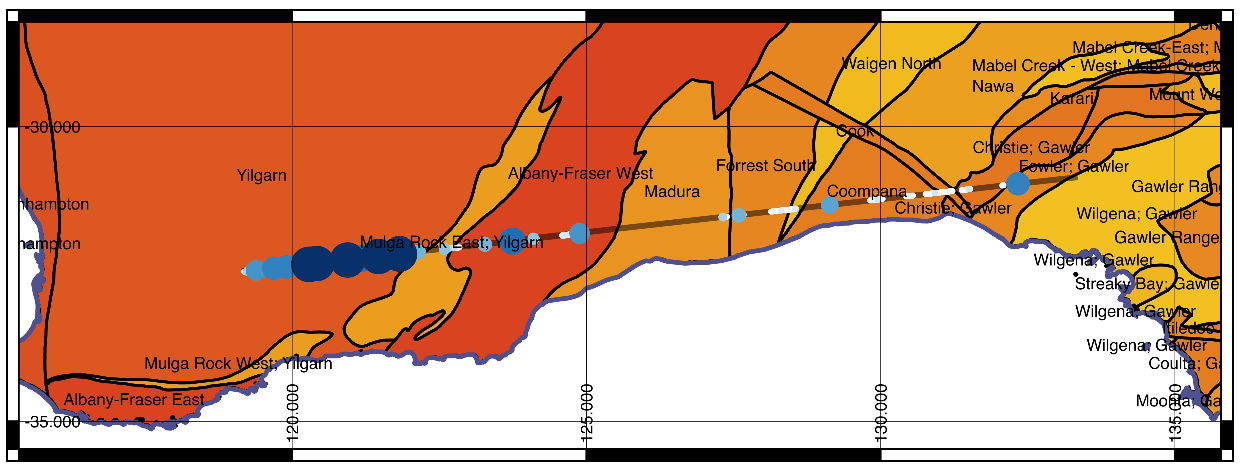
\includegraphics[width=0.78\linewidth]{../fig/maps/Line_16_S5_T100}
			\caption{}
			\label{fig:Ng1} 
		\end{subfigure}

		\begin{subfigure}[b]{1\textwidth}
			\centering
			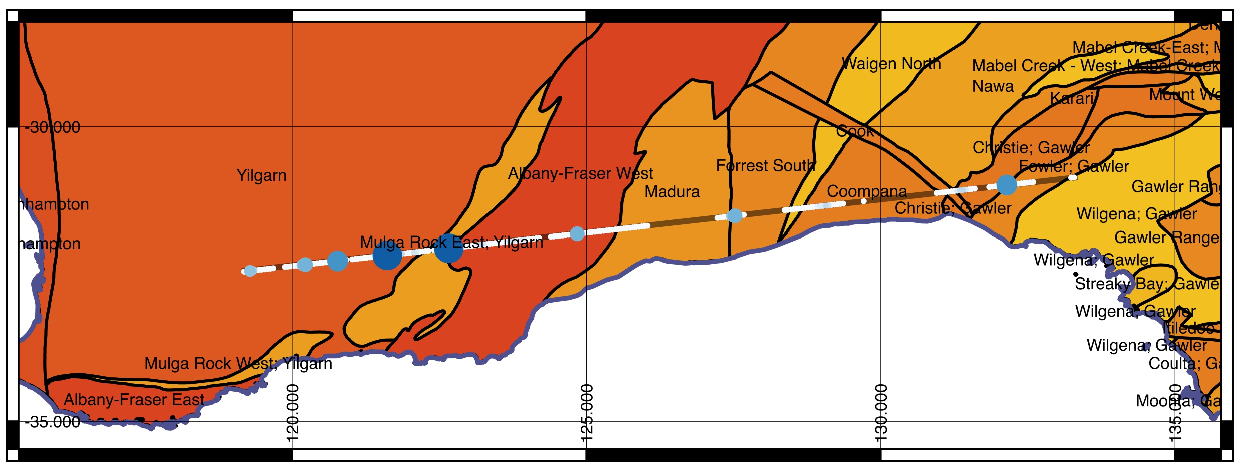
\includegraphics[width=0.78\linewidth]{../fig/maps/Line_16_S50_T100}
			\caption{}
			\label{fig:Ng2}
		\end{subfigure}

		
		\begin{subfigure}[b]{1\textwidth}
			\centering
			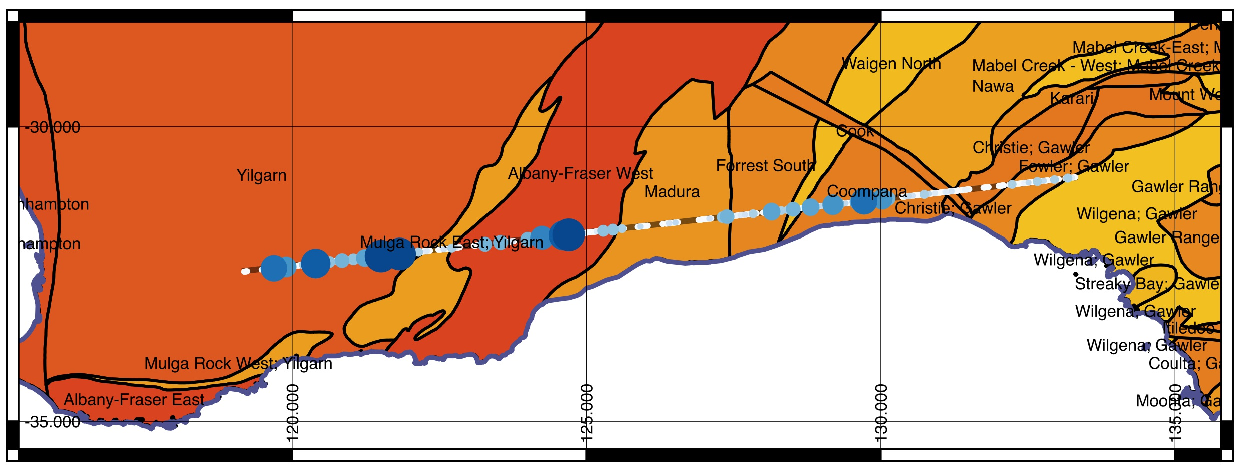
\includegraphics[width=0.78\linewidth]{../fig/maps/Line_16_S5_T100_No_Radio}
			\caption{}
			\label{fig:Ng3}
		\end{subfigure}
		
		\begin{subfigure}[b]{1\textwidth}
			\centering
			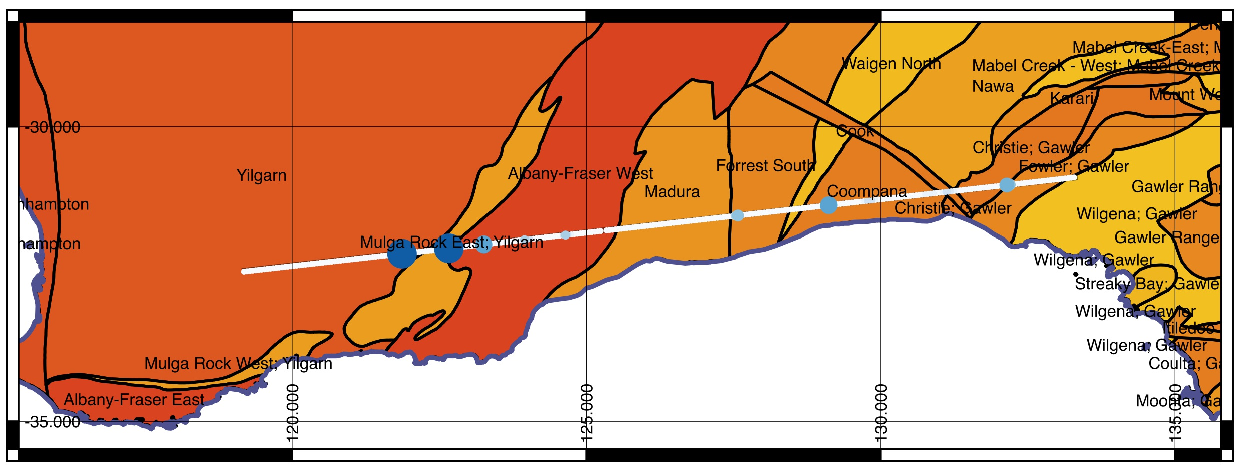
\includegraphics[width=0.78\linewidth]{../fig/maps/Line_16_S50_T100_No_Radio}
			\caption{}
			\label{fig:Ng4}
		\end{subfigure}		
		

		\caption[Resampling and radiometry compararasion for Line 16]{Line 16 (a) Sub-sampled 1:5, all parameters (b) Sub-sampled 1:50. (c) No radiometric data, sub-sampled 1:5 (d) No radiometric data sub-sampled 1:50. The dots symbolise probability (Pcp), darker. Smallest white is $10^-6$ and largest dark blue is $1$. See plots for exact values. }
	\end{figure}


\begin{sidewaysfigure}
	\centering


\centering
\includegraphics[width=1\linewidth]{"../fig/maps/All lines"}
\caption[Change points for all lines]{Lines subsampled 1:5. Changepoints calculated from gravity, magnetic and radiometric (K, Th and U).}
\label{fig:all-lines}

\end{sidewaysfigure}


\begin{sidewaysfigure}
	\centering
	
	
	\centering
	\includegraphics[width=1\linewidth]{"../fig/maps/slope_of_slope"}
	\caption[Derivate of changes in magnetic potential field.]{This map shows the derivative of changes in the magnetic potential field. Gawler, Musgrave and Yilgarn is well recognizable. This is an example of tests of 2D datasets to guide interpolation of change-points. Moreover, the steep second order derivatives relates to the background noise or spikiness in the change-point detection for catatonic areas with short sample length.}
	\label{fig:slopes}
	
\end{sidewaysfigure}


\begin{sidewaysfigure}
	\centering
	
	\centering
	\includegraphics[width=1\linewidth]{"../fig/maps/rough_change"}
	\caption[Derivate of changes in magnetic potential field and suggested changepoints.]{Roughness and detected change-points.}
	\label{fig:slopes_and_change}
	
\end{sidewaysfigure}